\chapter{Cell assembly analysis}
\label{chap:AssemblyAnalysis}
In this chapter we present the assembly analysis conducted on the data set introduced in \hyperref[sec:Dataset]{Section~\ref*{sec:Dataset}}, using the cell assembly detection algorithm and the single units classification presented in \hyperref[chap:AssemblyMethod]{Chapter~\ref*{chap:AssemblyMethod}} and \hyperref[chap:UnitsAnalysis]{Chapter~\ref*{chap:UnitsAnalysis}} respectively.\\
The cell assembly detection algorithm is designed to detect any coordinated spike trains patterns at any time scale. The time scales were explored running over different bin-widths. Further we examined the lag distribution. Lags describe the temporal distance in activation between units in assembly. Applying the cell-assembly algorithm we detected synchronous ($lag=0$) and asynchronous ($lag\neq0$) cell assemblies at arbitrary time scale ($\Delta$).\\Being interested in cross areal interactions and directionality between ventral striatum (VS) and ventral Tegmental area (VTA), we focused our study on interregional assembly-pairs, that are formed by two neurons, of which one neuron is located in the VS and the other one in VTA. At the pair-level, the lag in activation between units in assembly indicates the lag in activation between the two regions. A positive lag ($lag>0$) indicates that the VS unit is preceding in its activation the VTA unit, or in other words: VS is leading and VTA is following. A negative lag ($lag<0$) means that the VTA unit is preceding the activation of the VS unit, hence VTA is leading and VS is following.
\section{Cell types occurrence}
\label{sec:AsseTypes}
Based on the unit classification (\hyperref[chap:UnitsAnalysis]{Chapter~ \ref*{chap:UnitsAnalysis}}), interregional assembly were classified according to their underlying cell-types (figure \ref{fig:PieAssembliesTot} (B.)).
\begin{figure}[H]
    \centering
    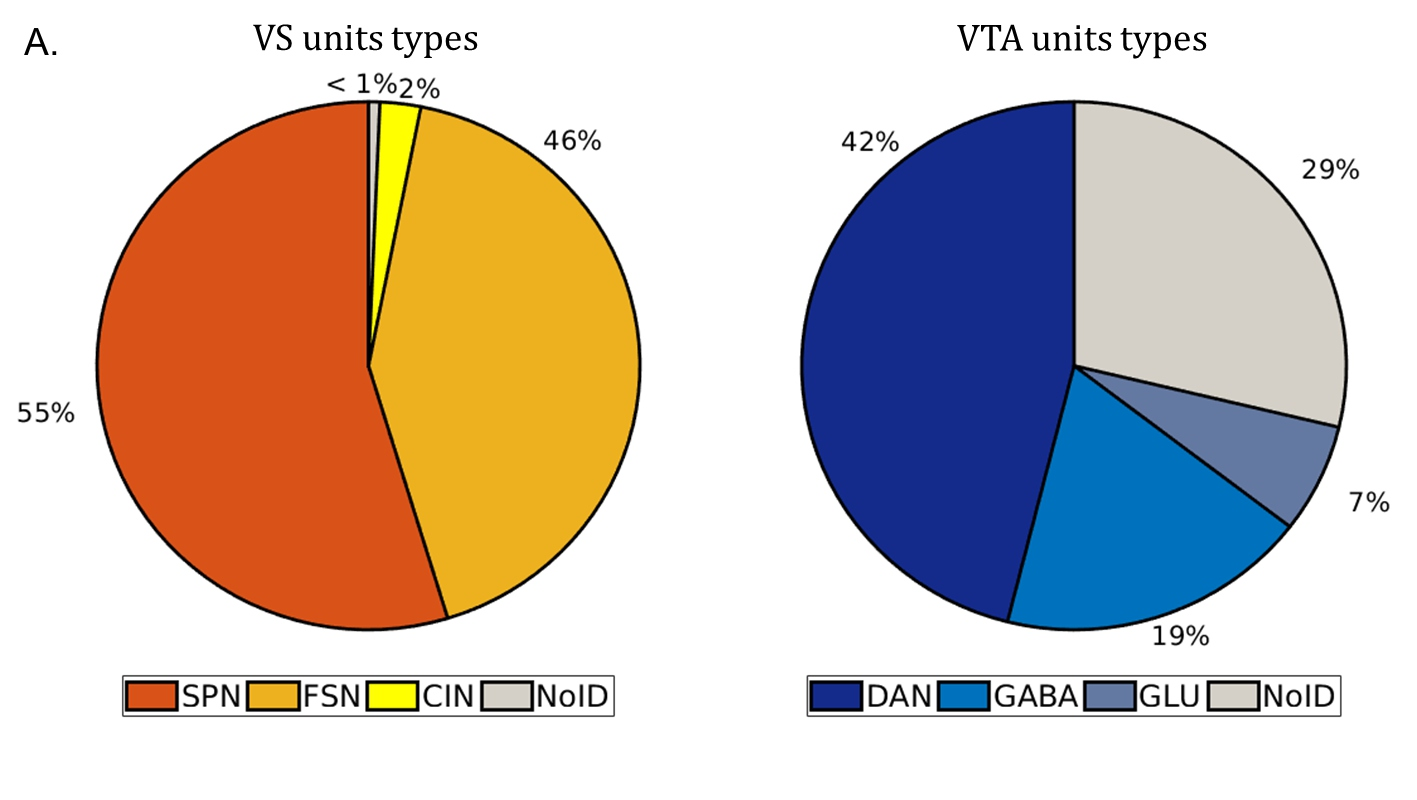
\includegraphics[scale=0.35]{figures/PieRegions1.pdf}
    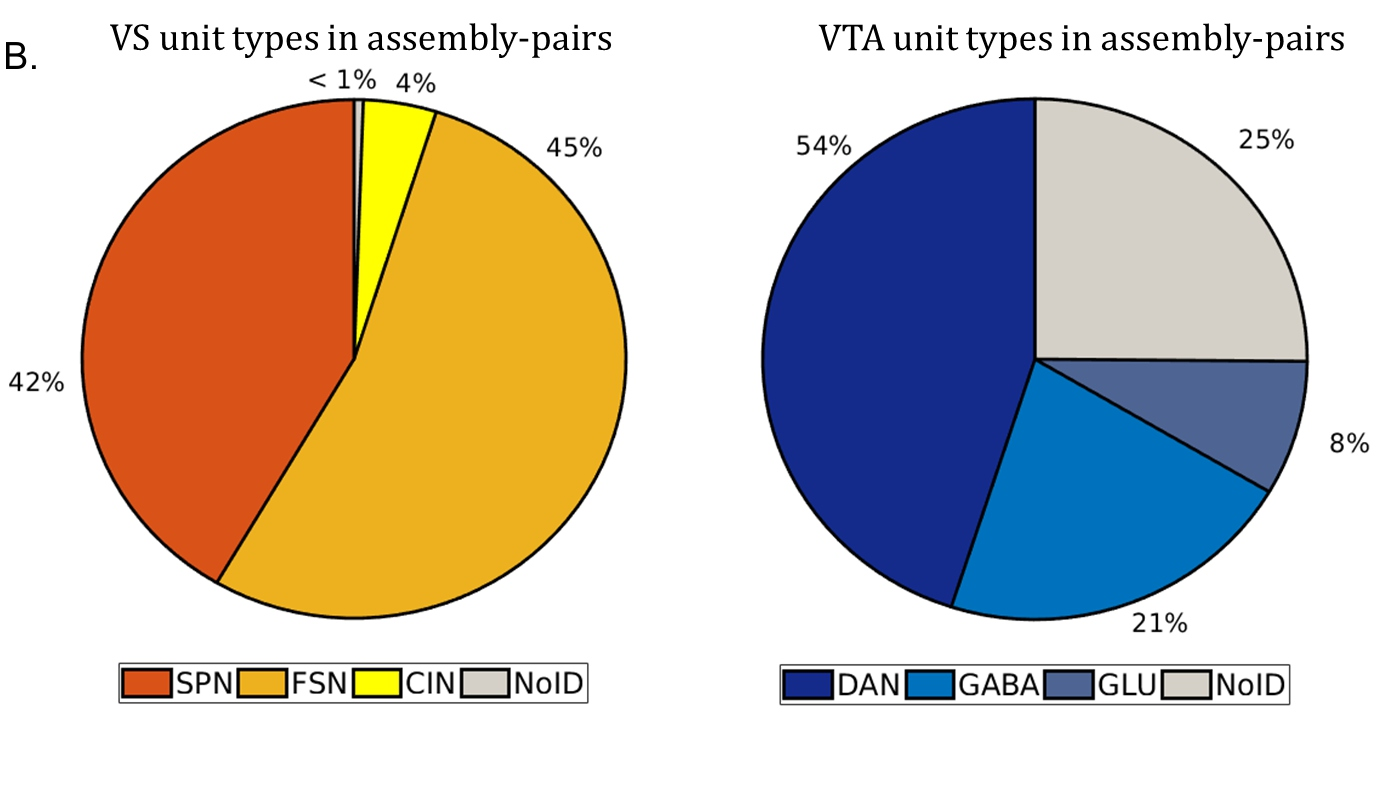
\includegraphics[scale=0.35]{figures/PieAsNotAs.pdf}
    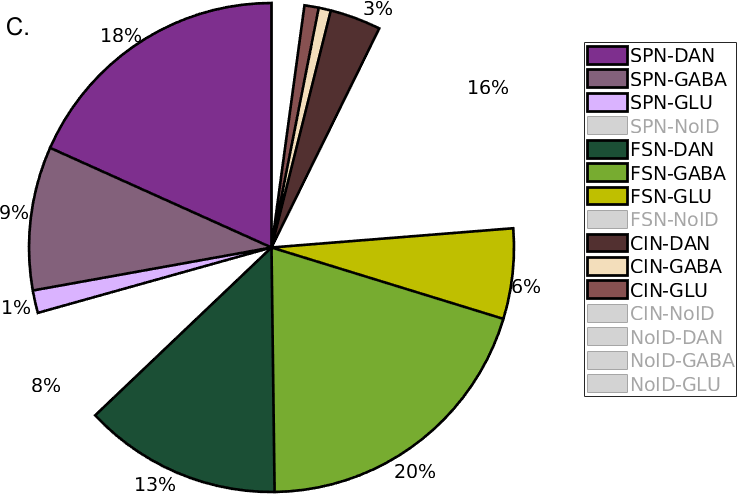
\includegraphics[scale=0.35]{figures/PieAssembliesTot1.png}
    \caption{(A.) Occurrence of classified and non-classified units in VS and VTA. (B.) Occurrence of classified and non-classified units of VS and VTA in interregional assembly-pairs. In VS, FSN occur in interregional pairs more often than SPN, even though more SPN than FSN were recorded.(C.) Pie charts of assemblies types. Cell types with $<1\%$ are not indicated. Missing pieces of cake indicates pairs that include non-classified units. The four more frequent interregional pairs, including only classified units, are pairs between fast spiking and gabaergic neurons ($20\%$), striatal projection neurons and dopamine neurons ($18\%$), fast spiking and dopamine units ($13\%$), and striatal projection and gabaergic units ($9\%$). }
    \label{fig:PieAssembliesTot}
\end{figure}
Comparing the two pie charts related to the VS region (figure \ref{fig:PieAssembliesTot} (A. vs B.)), one observes that fast spiking neurons (FSN) occurred in interregional pairs more often than striatal projection neurons (SPN) (figure \ref{fig:PieAssembliesTot} (B.-left)), even though in the total sample of recorded neurons FSN are less frequent than SPN (figure \ref{fig:PieAssembliesTot} (A.-left)).
\label{sec:CellTypesOcc}
We hypothesized that specific cell-types had a higher tendency to aggregate into cell assemblies; to verify this hypothesis, we conducted for each of the two regions a Pearson's $\chi^2$ test. Of the classified unit types, only the ones detected at sufficient frequencies could be tested for reasons of statistical power: namely putative striatal projection neurons (pSPN) and fast spiking neurons (FSN) in VS, and dopamine (DAN) and gabaergic (GABA) units in VTA. Only few striatal cholinergic interneurons and VTA glutamatergic units were detected in the examined data-set, and therefore not amenable to statistical analysis. We therefore focused on the four most prominent neuron types and the cell assembly pairs formed between those units.
\begin{table}[H]
    %\centering
\begin{tabular}{ |p{3cm}|p{3cm}|p{3cm}| }
 \hline
 \multicolumn{3}{|c|}{Pearson$'$s $\chi^2$ test VS unit type and interregional pair relationship} \\
 \hline
 & In pairs & Not in pairs\\
 \hline
 SPN & 153 (197.64) & 253 (208.36) \\
 \hline
 FSN & \textbf{197 (156.36)} & 116 (164.64)\\
 \hline
 \multicolumn{3}{|c|}{$\chi^2$ statistic  45.13}\\
 \multicolumn{3}{|c|}{p-value = $1.8\times10^{-11}$}\\
 \hline
 \multicolumn{3}{|c|}{$\chi^2$ statistic Yates correction 44.12}\\
 \multicolumn{3}{|c|}{p-value = $3.1\times10^{-11}$}\\
 \hline
\end{tabular}
\caption{Pearson's $\chi^2$ contingency table with $\chi^2$ value and p-value. Unit-types and interregional pairs formation are correlated in VS.}
\label{tab:chi2_asnotasVS}
\end{table}
\begin{table}[H]
    %\centering
\begin{tabular}{ |p{3cm}|p{3cm}|p{3cm}| }
 \hline
 \multicolumn{3}{|c|}{Pearson's $\chi^2$ test VTA unit-type and interregional pair relationship} \\
 \hline
 & In pairs & Not in pairs\\
 \hline
 DAN & 86 (90.604) & 31 (26.40) \\
 \hline
 GABA & 41 (36.40) & 6 (10.60)\\
 \hline
 \multicolumn{3}{|c|}{$\chi^2$ statistic  3.62}\\
 \multicolumn{3}{|c|}{p-value = 0.057}\\
 \hline
\end{tabular}
\caption{Pearson's $\chi^2$ contingency table with $\chi^2$ value and p-value. Unit-types and interregional pairs formation are not correlated in VTA.}
\label{tab:chi2_asnotasVTA}
\end{table}
Whether the recorded unit may or may not be part of an interregional pair is described  in the contingencies tables \ref{tab:chi2_asnotasVS}, \ref{tab:chi2_asnotasVTA}. In the contingencies tables, the number (compared to the expected values indicated in parentheses) of specific cell types in interregional pairs were reported with $\chi^2$ statistic p-values. For each test the $\alpha$ significance level was fixed at $0.05$, unless otherwise specified.\\
A relationship between unit types and interregional pairs formation was found only in VS. In VS the $\chi^2$ statistic value is 45.13 (44.12 using Yates correction), that gives a p-value of $1.8\times10^{-11}$ ($3.1\times10^{-11}$). The results confirmed that in VS the tendency of being agglomerate in interregional pairs depended on the specific cell-type. A similar test was conducted in VTA, with a resulting $\chi^2$ statistic of $3.62$ and a p-value of $0.057$, not significant at $\alpha = 0.05$ level. We therefore conclude that in VTA different cell-types had more comparable probabilities to agglomerate in interregional pairs.\\
We have shown above how often VS and VTA units occur in assemblies. We next analyzed if specific interregional pair-types occur systematically more often than others. The occurrence of assembly-types for the recorded units is shown in the pie-chart of figure \ref{fig:PieAssembliesTot} (bottom). Pieces of the pie chart without displayed percentages refer to pairs occurring with a rate below $< 1\%$.  Missing pieces of the pie chart indicate pairs that included non-classified units. Selecting only classified units, four assemblies types occurred more often than other, they were pairs formed by fast spiking and gabaergic neurons (20$\%$), striatal projection neurons and dopamine neurons (18$\%$), fast spiking and dopamine units (13$\%$) and striatal projection and gabaergic units (9$\%$).
\begin{table}[H]
    %\centering
\begin{tabular}{ |p{3cm}|p{3cm}|p{3cm}| }
 \hline
 \multicolumn{3}{|c|}{Pearson's $\chi^2$ test ($VS \rightarrow VTA$)} \\
 \hline
 & DAN pairs & GABA pairs\\
 \hline
 SPN & 76 (63.77) & 35 (47.23) \\
 \hline
 FSN & 32 (44.23) & 45 (32.77)\\
 \hline
 \multicolumn{3}{|c|}{$\chi^2$ statistic  13.47}\\
 \multicolumn{3}{|c|}{p-value = $2\times10^{-4}$}\\
 \hline
 \multicolumn{3}{|c|}{$\chi^2$ statistic Yates correction 12.39}\\
 \multicolumn{3}{|c|}{p-value = $4\times10^{-4}$}\\
 \hline
\end{tabular}
\caption{Pearson's $\chi^{2}$ test contingency table. We tested the dependency between the neuron type in VS and the neuron type in VTA with which the pair is formed, for pairs with specific directionality $VS \rightarrow VTA$. The $\chi^2$ test show a dependency among variables, meaning that specific pairs have higher tendency to agglomerate in assembly.}
\label{tab:chisquare_vsvta}
\end{table}
\begin{table}[H]
\begin{tabular}{ |p{3cm}|p{3cm}|p{3cm}| }
 \hline
 \multicolumn{3}{|c|}{Pearson$'$s $\chi^2$ test ($VS \leftarrow VTA$)} \\
 \hline
 & SPN pairs & FSN pairs\\
 \hline
 DAN & 18 (12.06) & 29 (34.94) \\
 \hline
 GABA & 11 (16.94) & 55 (49.06)\\
 \hline
 \multicolumn{3}{|c|}{$\chi^2$ statistic  6.73}\\
 \multicolumn{3}{|c|}{p-value = 0.009}\\
 \hline
 \multicolumn{3}{|c|}{$\chi^2$ statistic Yates correction 5.65}\\
 \multicolumn{3}{|c|}{p-value = 0.017}\\
 \hline
\end{tabular}
\caption{Pearson$'$s $\chi^{2}$ test contingency table. We tested the dependency between the neuron type in VTA and the neuron type in VS with which the pair is formed, for pairs with specific directionality $VS \leftarrow VTA$. The $\chi^2$ test show a dependency among variables, meaning that specific pairs have higher tendency to agglomerate in assembly.}
\label{tab:chisquare_vtavs}
\end{table}
To see whether assembly types occurred by chance and whether there was a relationship between the unit type activated in one region and the resulting assembly pairs, again a Pearson's $\chi^2$ test was conducted. Specifically, given the relative frequency of certain types of assemblies, we hypothesized a preference for fast spiking neurons with gabaergic neurons (and/or vice-versa) and a preference for striatal projection neurons with dopamine neurons (and/or vice-versa). The $\chi^2$ test were performed on the directional pairs ($lag\neq0$) and separately on $VS\rightarrow VTA$ ($lag>0$) and $VS\leftarrow VTA$ ($lag<0$). In both cases, the p-values of $\chi^2$ test were significant at the confidence level $\alpha = 0.05$, hence the $\chi^2$ test confirmed a dependence between the cell-type and the resulting interregional assembly pair type. In direction $VS\rightarrow VTA$ the p-value was $2\times10^{-4}$ ($p=4\times10^{-4}$ using Yates correction), in direction $VS\leftarrow VTA$: $p=9\times10^{-3}$ ($p=0.017$ using Yates correction). The contingency and the results of the $\chi^2$ tests are shown for the two directionalities in tables \ref{tab:chisquare_vsvta} and \ref{tab:chisquare_vtavs}. The activated cell types of the leading region are indicated in the rows, the coupled selected cell types of the follower region in the columns. In the table-elements the number of pairs between the two cell-types and in parenthesis the expected values. Both in $VS\rightarrow VTA$ and in $VS\leftarrow VTA$ directionalities the real values of couples $SPN+DAN$ and $FSN+GABA$ exceed the expected values. In both directionality specific pair-types have an higher tendency to occur.
\section{Inter-/intra- regional pair time scales}
\label{sec:TimeScales}
In the previous session we have seen that in VS the neuronal occurrence in assembly depends on the cell-types, and specifically (FSN) occur more frequently in assembly than (SPN). Furthermore we have seen that, in directional assemblies, the combination among cell types is non-random. With these analysis we described the cell types occurrence in VS-VTA interactions. Time scales involved in the cross-area interactions will be examined later in this chapter, together with a comparison with intra-area interaction time scales.\\
Detecting assemblies at any time scale, the detection algorithm dissects the time scales involved in interregional-interactions. A set of bin widths $\Delta \in \{\Delta_{min}...\Delta_{max}\}$ is provided as input, so that spike patterns can be detected at different bin-size, pairs are tested at all possible bin widths, then for each assembly, the width $\Delta^*$ associated with the lowest p-value is chosen as its characteristic temporal precision (\cite{RussoDurstewitz}, see \hyperref[chap:AssemblyMethod]{Chapter~ \ref*{chap:AssemblyMethod}}).\\
Figure \ref{fig:BinDistr} shows the temporal scale ($\Delta$) distribution of VS-VTA interregional-interactions. Figures \ref{fig:BinDistrVS} and \ref{fig:BinDistrVTA} show VS-VS and VTA-VTA time-scale interactions distribution respectively.
\begin{figure}[H]
%\centering
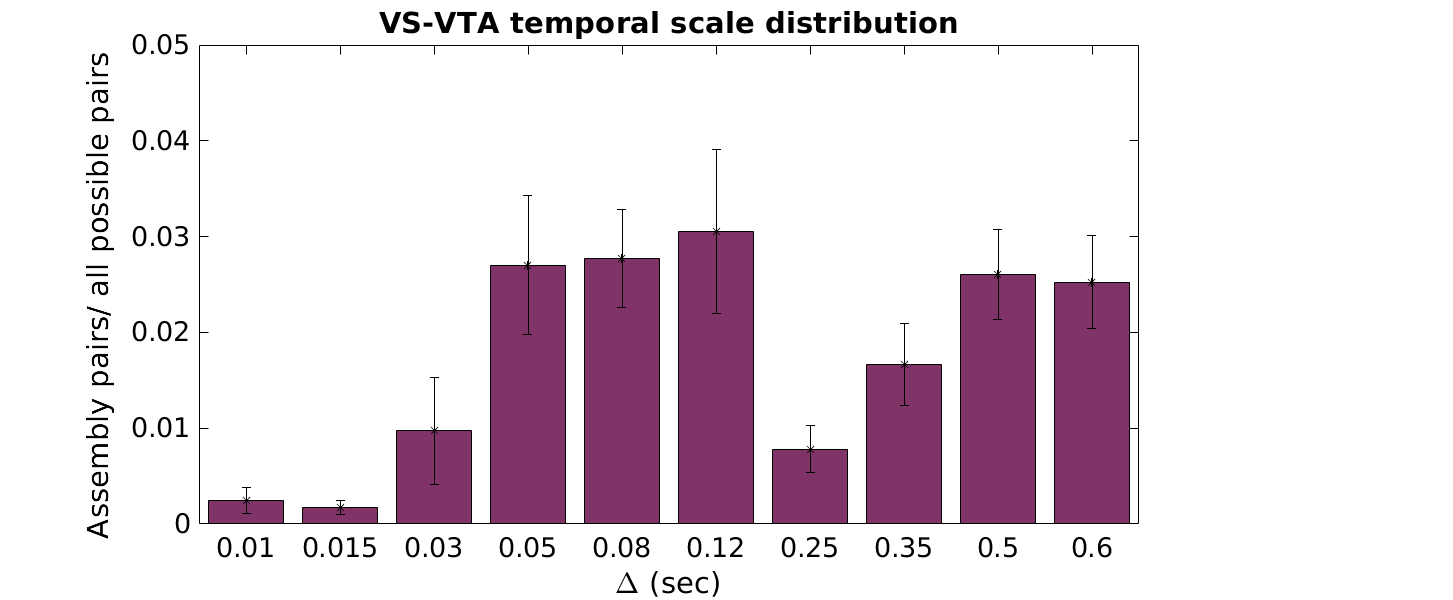
\includegraphics[scale=0.46]{figures/VS_VTA_Short1.png}
\caption{Bin distribution for interregional pairs. VS-VTA pairs show a bimodal distribution, revealing two temporal scales involved in interregional activation patterns.}
\label{fig:BinDistr}
\end{figure}
\begin{figure}[H]
%\centering
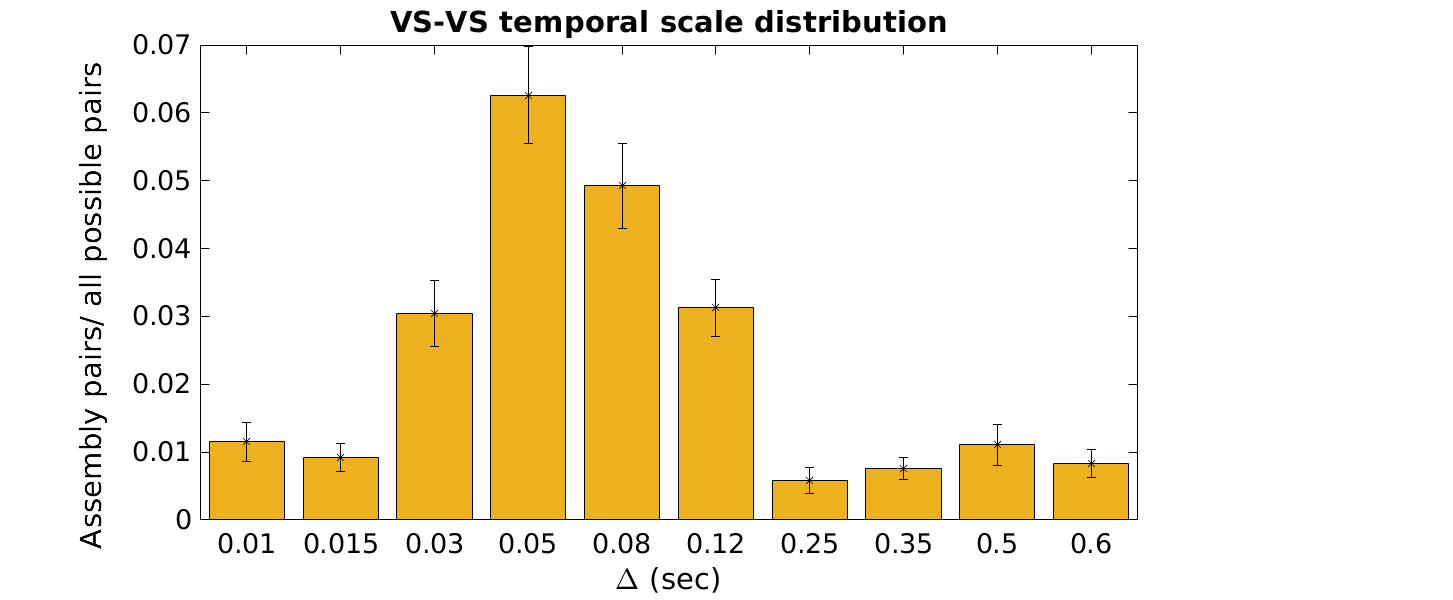
\includegraphics[scale=0.46]{figures/VS_VS_S.png}
\caption{VS-VS pairs are more precise than VS-VTA pairs and the bin distribution presented with a peak at 50 $ms$}
\label{fig:BinDistrVS}
\end{figure}
\begin{figure}[H]
%\centering
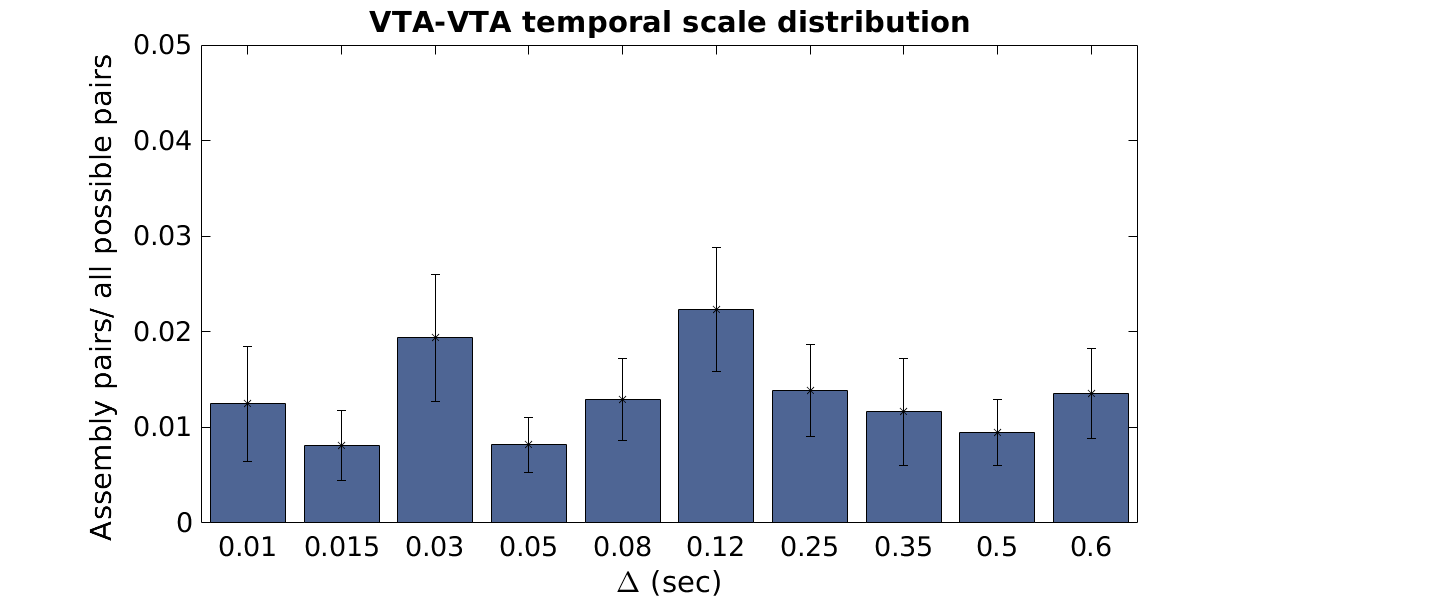
\includegraphics[scale=0.46]{figures/VTA_VTA_S.png}
\caption{VTA-VTA temporal scales were broadly distributed.}
\label{fig:BinDistrVTA}
\end{figure}
A comparison among interregional pairs (VS-VTA pairs) and intraregional pairs (VS-VS pairs and VTA-VTA pairs) show interesting differences:\\
while we observed assemblies with temporal precision at the scale of few tens of milliseconds only within either VS or VTA, assemblies of lower temporal precision were detected across VS-VTA units. Interregional VS-VTA interactions had a bimodal time-scales distribution with two peaks, one around 80 $ms$ and one at 1.6 $sec$, revealing two time scales involved in VS-VTA interaction. The first, more precise time scale, ranged from 10 $ms$ to 250 $ms$, and the second included broader bin sizes. Interregional pairs thus had a bimodal distribution in their temporal precision.\\Bimodality is a characteristic specific of VS-VTA interactions, not present in VTA-VTA, or VS-VS interactions: intraregional VTA-VTA pairs did not present any peak in time scales distribution, whereas intraregional VS-VS bin size distribution peaked around 50 $ms$.  
\subsection{SPN-FSN time scales interactions *}
\label{sec:SPN-FSN_Bin}
Fast spiking neurons population had a broad range of firing rates, and according to the firing rate, sub-populations of the neurons, classified as FSN, showed different characteristic in terms of time-scales of interactions, or/and feature coding ({\color{red}ask for paper to cite}).\\From the distribution of mean firing rates of the recorded FSN was possible to define two sub-populations, those latter did not present different characteristic when their units are coupled in assembly with a VTA neuron; however FSN differ in relation to their time-scales interactions in intraregional pairs with SPN. FSN can be distinguished in two sub-populations based on their firing rate, FSN$^{low}$ and FSN$^{high}$: the first characterized to have mean firing rate below 45 Hz and the latter has mean firing rate equal or above 45 Hz (figure \ref{fig:FSNsFireHisto}).\\
\begin{figure}
    \centering
    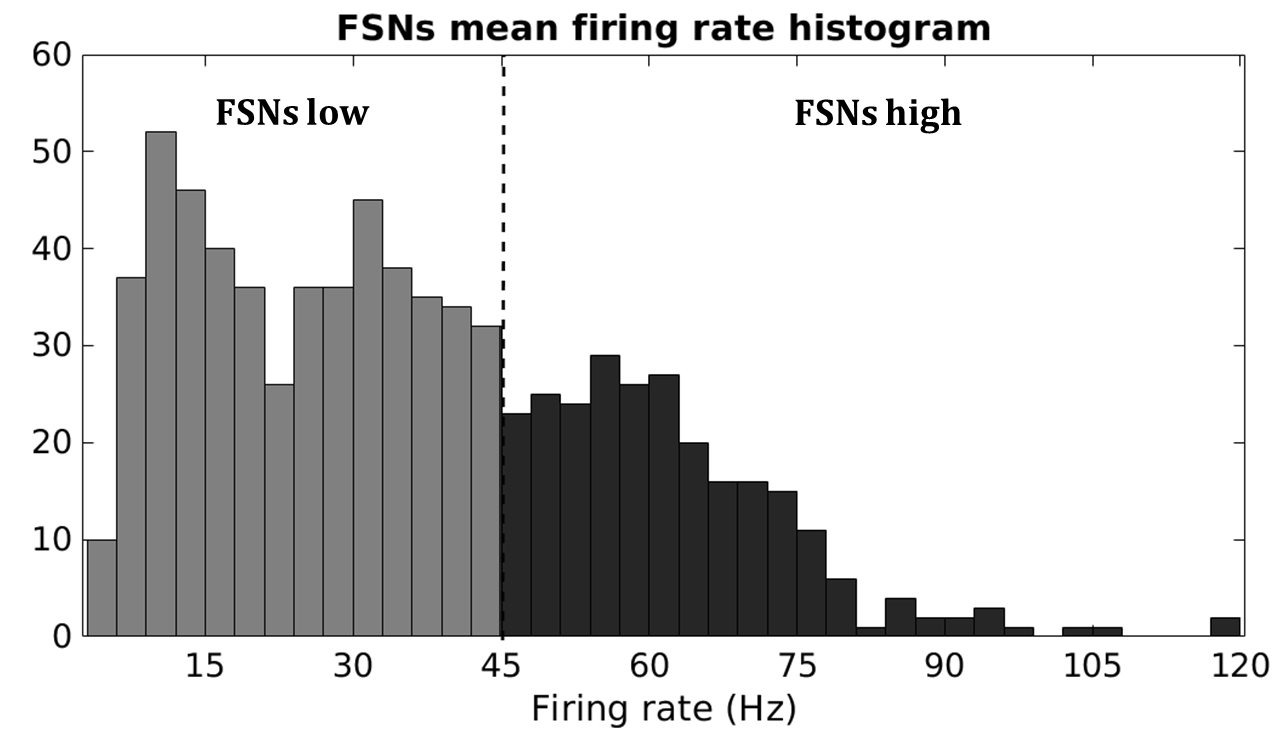
\includegraphics[scale=0.6]{figures/FSNFiringRateLightDark.pdf}
    \caption{Histogram of FSNs mean firing rate. We can distinguish two populations of FSNs: FSN$^{low}$ population, that are light grey in the graph, characterized by having firing rates below 45 Hz, FSN$^{high}$, in dark grey, characterized by having firing rates from 45 Hz upwards.}
    \label{fig:FSNsFireHisto}
\end{figure}
\begin{figure}
    \centering
    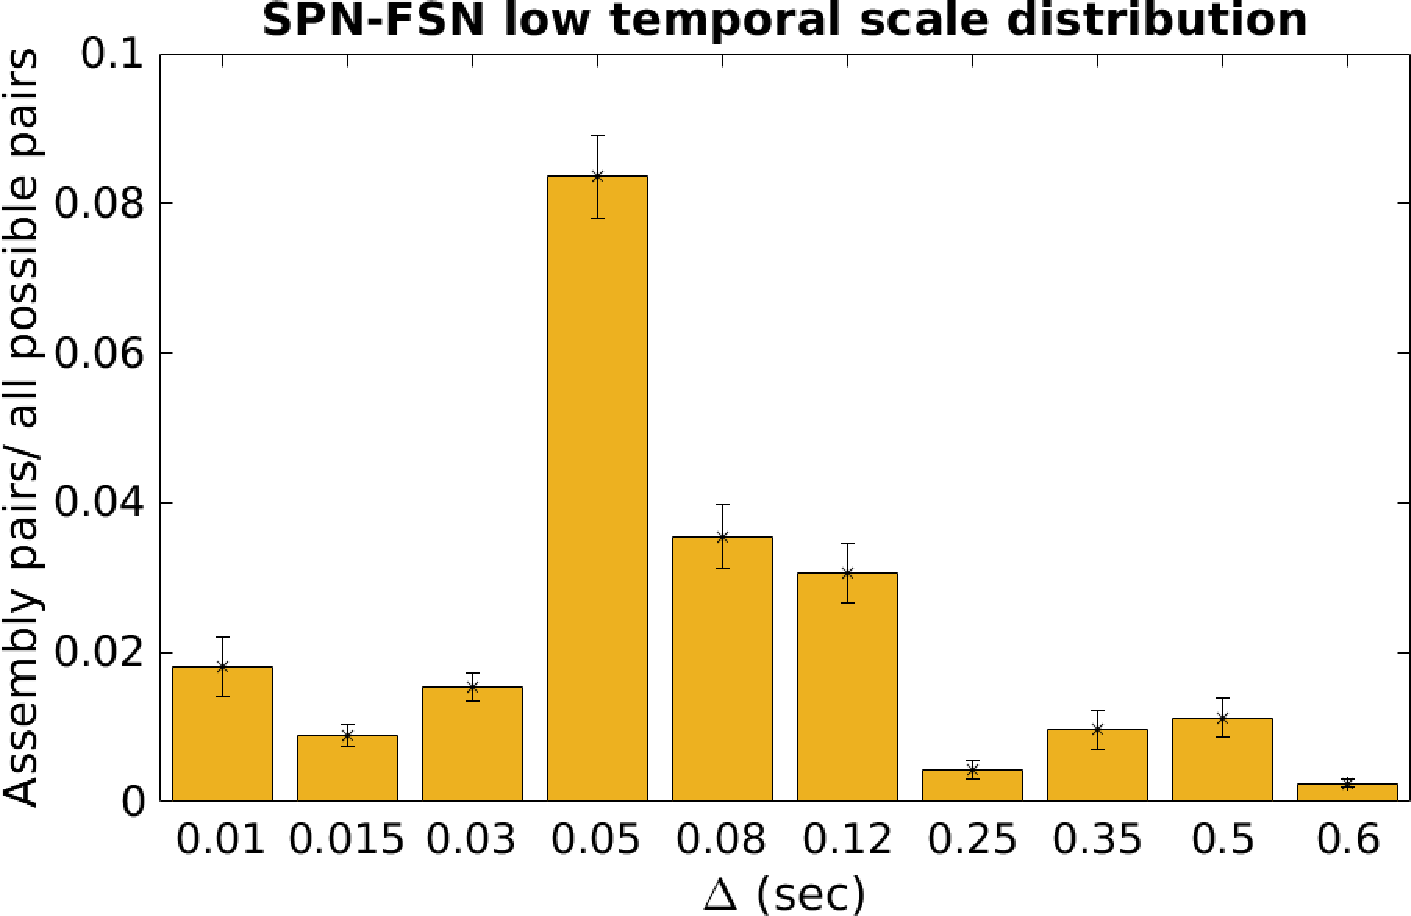
\includegraphics[scale=0.5]{figures/SPN_FSNlow1.pdf}
    \caption{SPN-FSN$^{low}$ temporal scale distribution peaked at 50 $ms$. With other frequent SPN-FSN$^{low}$ pairs detected also at 80 $ms$ and 120 $ms$.}
    \label{fig:SPN_FSNlowBin}
\end{figure}
\begin{figure}
    \centering
    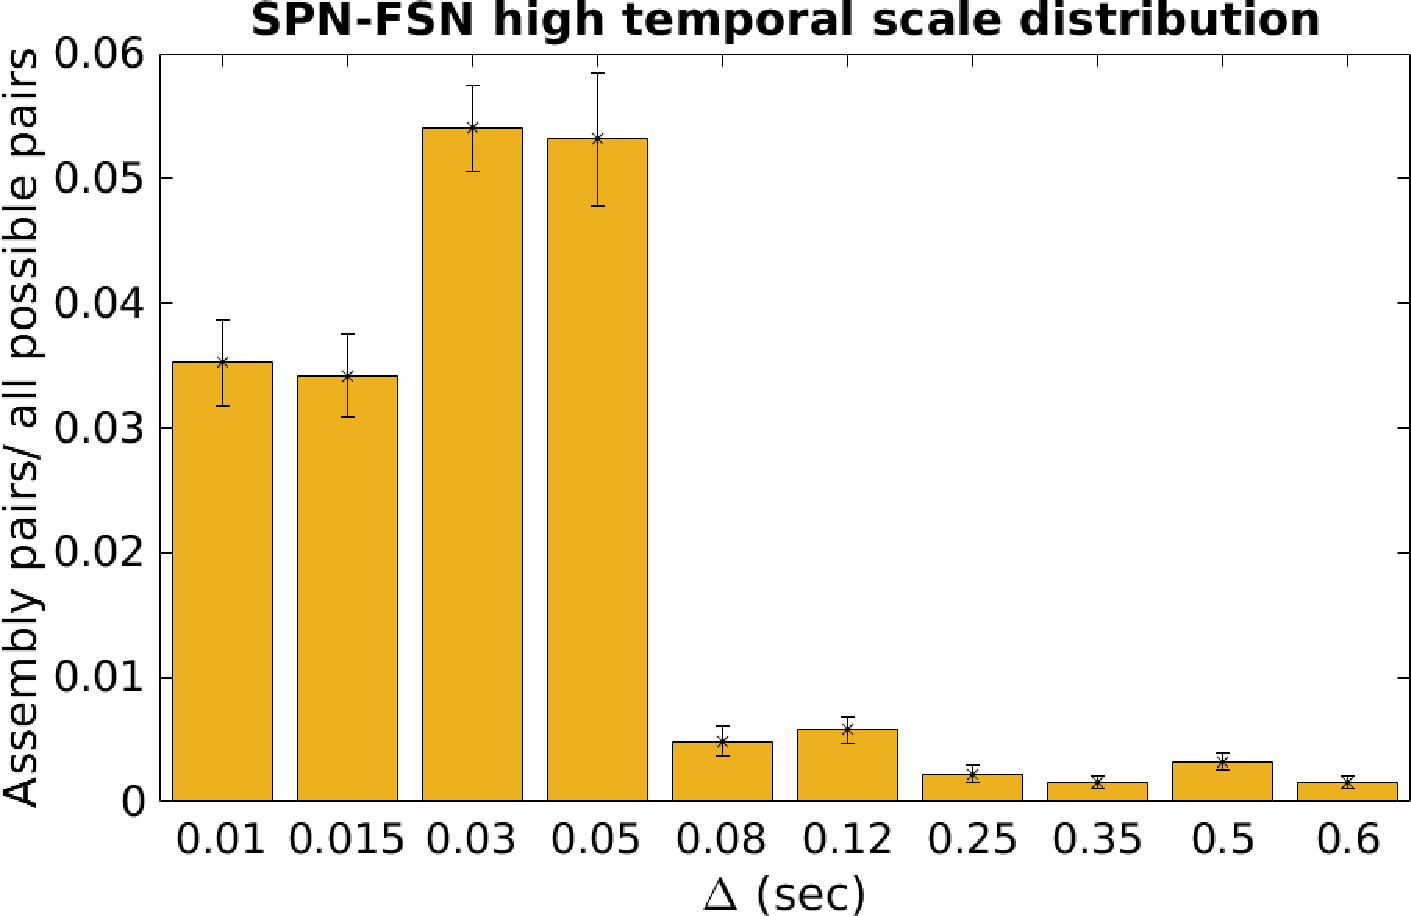
\includegraphics[scale=0.5]{figures/SPN_FSNhigh1.pdf}
    \caption{SPN-FSN$^{high}$ pairs were almost exclusively detected at very precise time scales, namely from 10 $ms$ to 50 $ms$.}
    \label{fig:SPN_FSNhighBin}
\end{figure}
In VS we noticed differences between SPN-FSN$^{low}$ pairs and SPN-FSN$^{high}$ bin size distributions. SPN-FSN$^{low}$ bin distribution pair is peaked at 50 $ms$, and another good portion of those pairs is detected at the two next bin sizes after the peak, 80 $ms$ and 120 $ms$ (figure \ref{fig:SPN_FSNlowBin}); whereas SPN-FSN$^{high}$ pairs are by-and-large only detected at more precise temporal scale (figure \ref{fig:SPN_FSNhighBin}).\\We conclude that those two pair-types give specific contributions to the global VS-VS temporal scale distribution. The variety of time scales involved in intra- or cross- area interactions in the studied regions emphasizes the complexity of the interaction circuit.
\section{Directionality} 
\label{sec:Directionality}
We had found in \hyperref[sec:TimeScales]{Section~\ref*{sec:TimeScales}} that interregional interactions have two characteristic time scales, which led us to consider more precise ($\Delta \in [0.01,0.25] ms$) and broader ($\Delta \in [0.25,0.6] ms$) time scales separately when examining the directionality of VS-VTA assembly-pairs.\\We recall that one of the output of the cell-assembly algorithm (CAD) is the inter-units activation lag of the assembly. When we restrict the investigation to interregional pairs, the lag value tells us the distance in activation between the two region while the sign of the lag indicates the direction of the activation, namely which region became activated first and which one follows.\\In figure \ref{fig:LagInSecAll} we show the lag distribution for detected interregional assembly-pairs in the two characteristic time scales of interaction. As indicated in the plot, a positive lag means that VS is functionally leading the VTA activation and a negative lag indicates the opposite direction.\\Interestingly lag distributions of precise pairs was asymmetric, indicating that preferentially the VS activation lead the activation of the VTA in that range of time scales. The two lag distributions showed remarkable differences: the lag distribution of broader pairs was fat-long tailed, indeed, a good portion of assembly-pairs detected had long activation lag ($lag > 1 sec$); more precise lag distribution had instead thin tails: almost all pairs detected in precise time scale had short lag ($|lag| < 1 sec$), and a good portion of pairs was detected within a lag value of 0.5 $sec$.\\
We focused the study on the more precise temporal scale, first because in such a way the temporal scale interactions were separated to typical task-related time scales, as e.g. the length of the odor duration, which covered typically an interval from 1.0 $sec$ to 1.5 $sec$. Secondly, the prediction error functions are expressed by dopamine circuit in short time scales (within 1 $sec$ from stimulus onset).\\ We used the cell-types classification presented in\hyperref[chap:UnitsAnalysis]{~Section \ref*{chap:UnitsAnalysis}} to divide the interregional assembly-pairs in assembly-pair types, according to their underlying cell-types (see \hyperref[sec:AsseTypes]{~Section \ref*{sec:AsseTypes}}). Doing so, we could divide the global lag distribution in lag distributions specific of those assembly-pairs types. Figure \ref{fig:LagInSec4typo} shows the lag distribution for the four principal assembly-pair types.\\
We observed that the directional assemblies are composed of striatal projection neurons leading dopamine neurons (SPN-DAN pairs), all the other pair-types do not show a clear preferred directionality. Furthermore, inter-unit activation lags of assemblies containing pallidal neurons (FSN) were shorter than those containing SPN, compatibly with assumed connectivity.\\
VTA dopamine neurons were laser tagged in first place, we can use the laser tagged units as control to validate the dopamine neurons classification. Figure \ref{fig:LagInSecLaser} shows the lag distribution of laser tagged dopamine units coupled with SPN and FSN. Similar lag distributions were observed for pairs containing laser tagged DAN and pairs containing all DAN based on response classification. Indeed, SPN-DAN$^{laser}$ pairs showed directionality in direction $VS\rightarrow VTA$, whereas FSN-DAN$^{laser}$ are not directional, as we expected from the results obtained using units selected by the classification criteria, which confirms the validity of the adopted classification.\\
\begin{figure}[H]
\centering
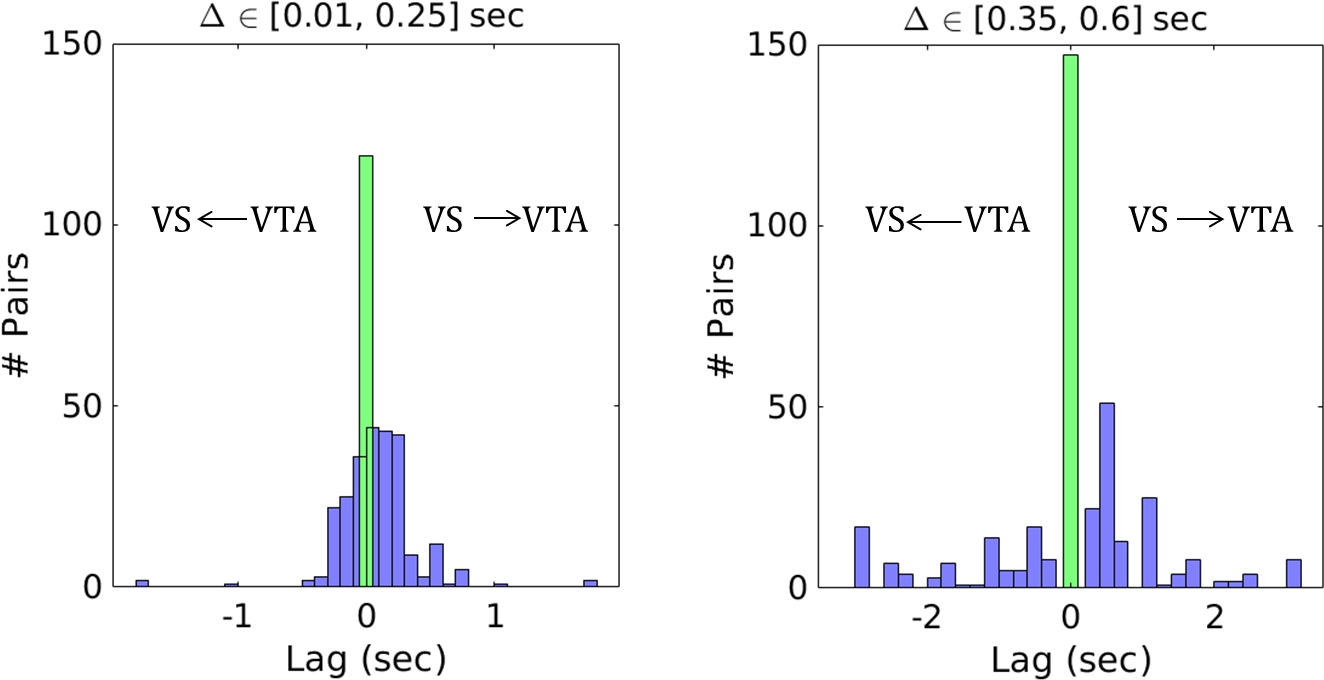
\includegraphics[scale=0.58]{figures/LagGeneral1.pdf}
\caption{Lag distribution for VS-VTA pairs in seconds. In green, the synchronous pairs. In violet, directional pairs. On the left, lag distribution of pairs detected in more precise time scale. Slight distribution asymmetry indicates directionality in the direction of $lag > 0$, meaning a predominance of pairs in which VS leads VTA. On the right, the lag distribution for pairs detected in the broader time scale, presented with a fat-tailed distribution.}
\label{fig:LagInSecAll}
\end{figure}
\begin{figure}[H]
\centering
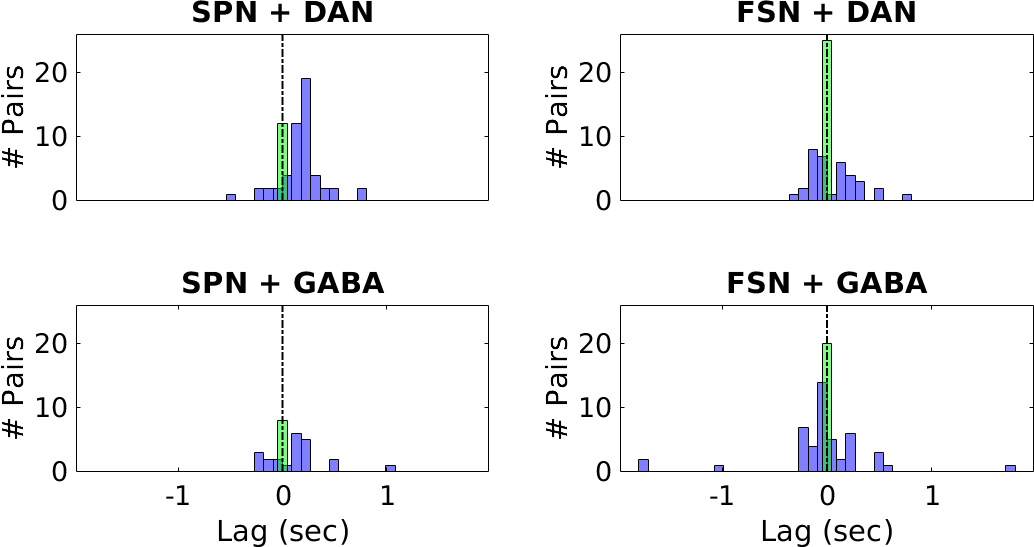
\includegraphics[scale=0.48]{figures/LagSec4Typo3VS.png}
\caption{Lag distribution of four more represented pair-types in precise time scale. Only SPN-DAN pairs show a preferred directionality, namely $VS\rightarrow VTA$.}
\label{fig:LagInSec4typo}
\end{figure}
\begin{figure}[H]
\centering
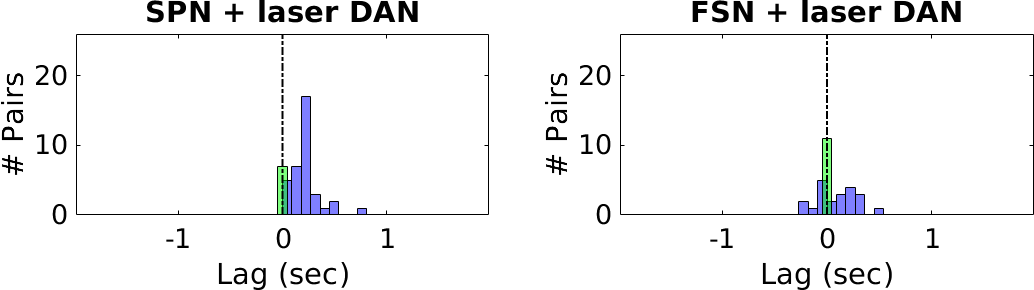
\includegraphics[scale=0.48]{figures/LagSecLaser3VS.png}
%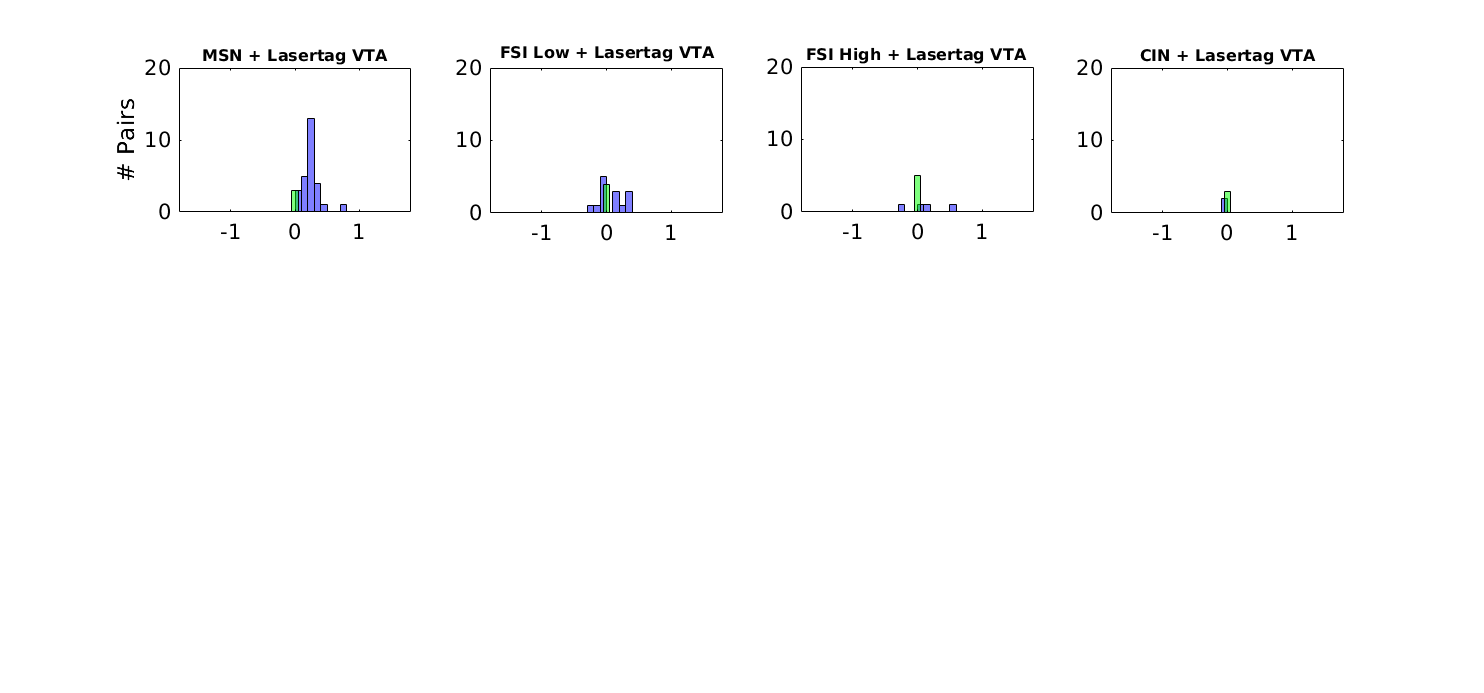
\includegraphics[scale=0.4]{figures/OnlyLaserOriz.png}
\caption{Lag distribution of DAN$^{laser}$ in pair with SPN and FSN units, in precise time scales. Lag distributions were similar to the lag distributions of classified DAN in pairs with SPN and FSN, confirming the directionality expressed by SPN-DAN pairs and the validity of the classification adopted in VTA.}
\label{fig:LagInSecLaser}
\end{figure}
The kind of activation exhibited by directional pairs is exemplified in figure \ref{fig:directional_assembly}. The pair in the example was detected with a bin width of $\Delta = 0.12 sec$, and the inter-units activation lag was positive $lag = 0.36 sec$. From the activation profile and the separation between the two activation one can see that the illustrated assembly-pair specifically coded for the rewarded odor.\\
Finally, looking at the activity of two neurons, the directionality exemplified by the pair was evident: first the VS unit became actived and, after a temporal delay, the activation of VTA unit followed. Raster plots show how the activity across trials changed. In both units we see a gradient of activation across trials. In first trials (less than 10 trials) the activity was either rare (VS unit), or uniform distributed in the odor window (VTA unit); after few trials, VS unit first, and later the VTA unit, showed a peak in activation at odor onset, that, then remained stable.\\ 
\begin{figure}
    \centering
    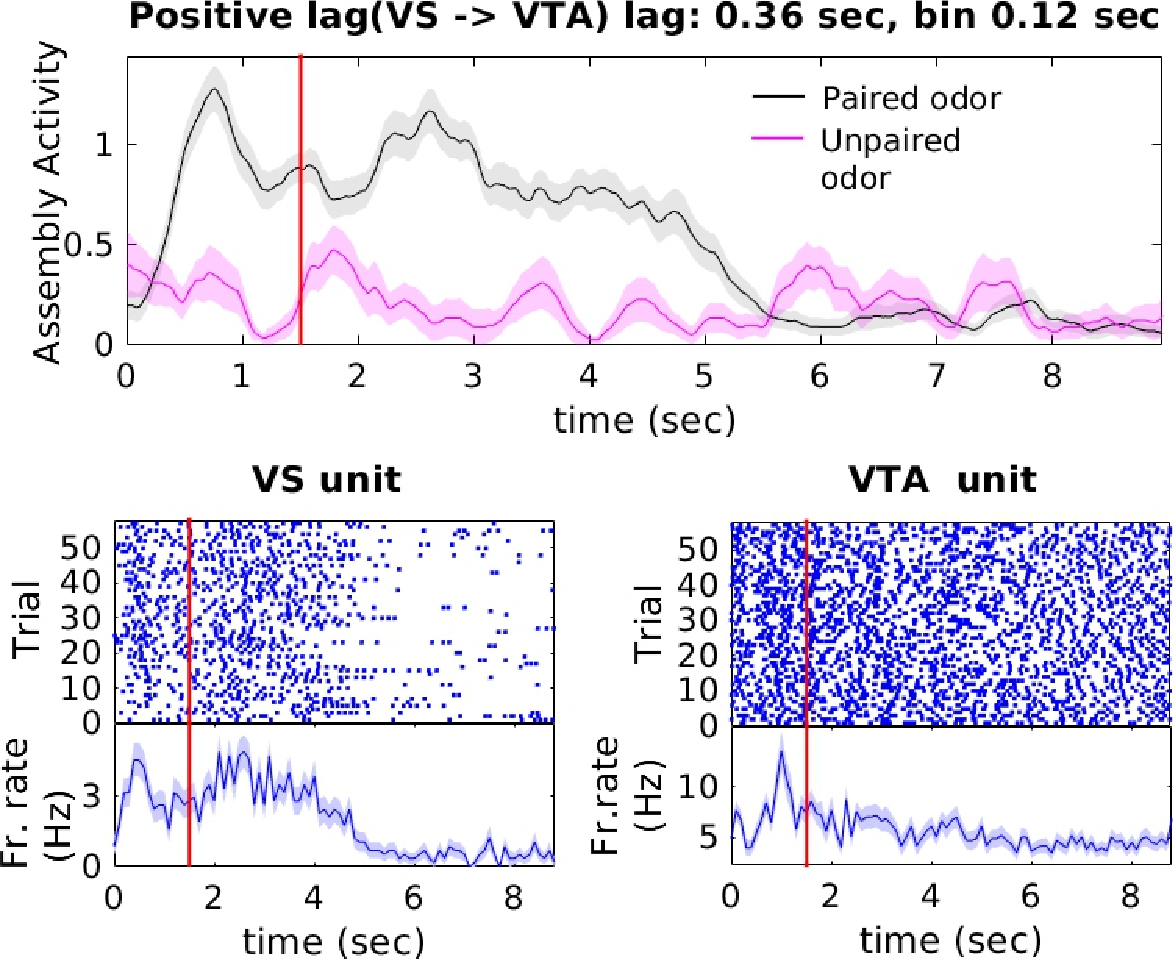
\includegraphics[scale=0.6]{figures/DirectionalAsEx1.pdf}
    \caption{Directional assembly.\textbf{Top:} mean across trails and standard error of the activity of the pair for the rewarded (grey) and unrewarded odor (purple) in the original phase. \textbf{Bottom:} raster plot and firing rate (mean and standard deviation) of units in an exemplary assembly-pair. x-axis origin corresponds to the odor onset, while the red line marks the end of the stimulus duration. The examined assembly had a positive lag, that means VS preceding in activity VTA. In the neuronal firing activity the VS unit activated before than the VTA unit.}
    \label{fig:directional_assembly}
\end{figure}
At population level, time scale and directionality segregation revealed different assembly-activation patterns. In figure \ref{fig:AsActBinLag} an example of activation patterns is shown for the interregional assembly-pairs activity averaged across trials\footnote{The activation $\mathcal{I}$ ranges in the interval $[0,1]$, after normalized as follows:
\begin{equation}
    \mathcal{I} = \frac{I-\min(I)}{\max(I)-\min(I)}
    \label{eq:norm}
\end{equation}}. 
Assembly-pairs exhibiting directionality $VS \rightarrow VTA$ and detected in the precise time scale ($\Delta \le 0.25$) became activated early during the odor presentation.\\The early activation at the stimulus presentation is the type of activation we expected when the animal predicts the reward. As discussed in \hyperref[sec:StateArt]{Section~\ref*{sec:StateArt}} (see also figure \ref{fig:Fiorillo}), reward-related responses in DAN changed as the reward probability change. The typical prediction error signal is presented as an high activation at the stimulus presentation in case of high reward probability, and less activation at the retrieval. Moreover we have shown in figure \ref{fig:LagInSec4typo} that the SPN-DAN assembly-pairs were directional, thus we speculated that SPN-DAN were good candidate for reward prediction error coding; the investigation of this hypothesis will be argument of the next chapters.\\
\begin{figure}[h!]
    \centering
    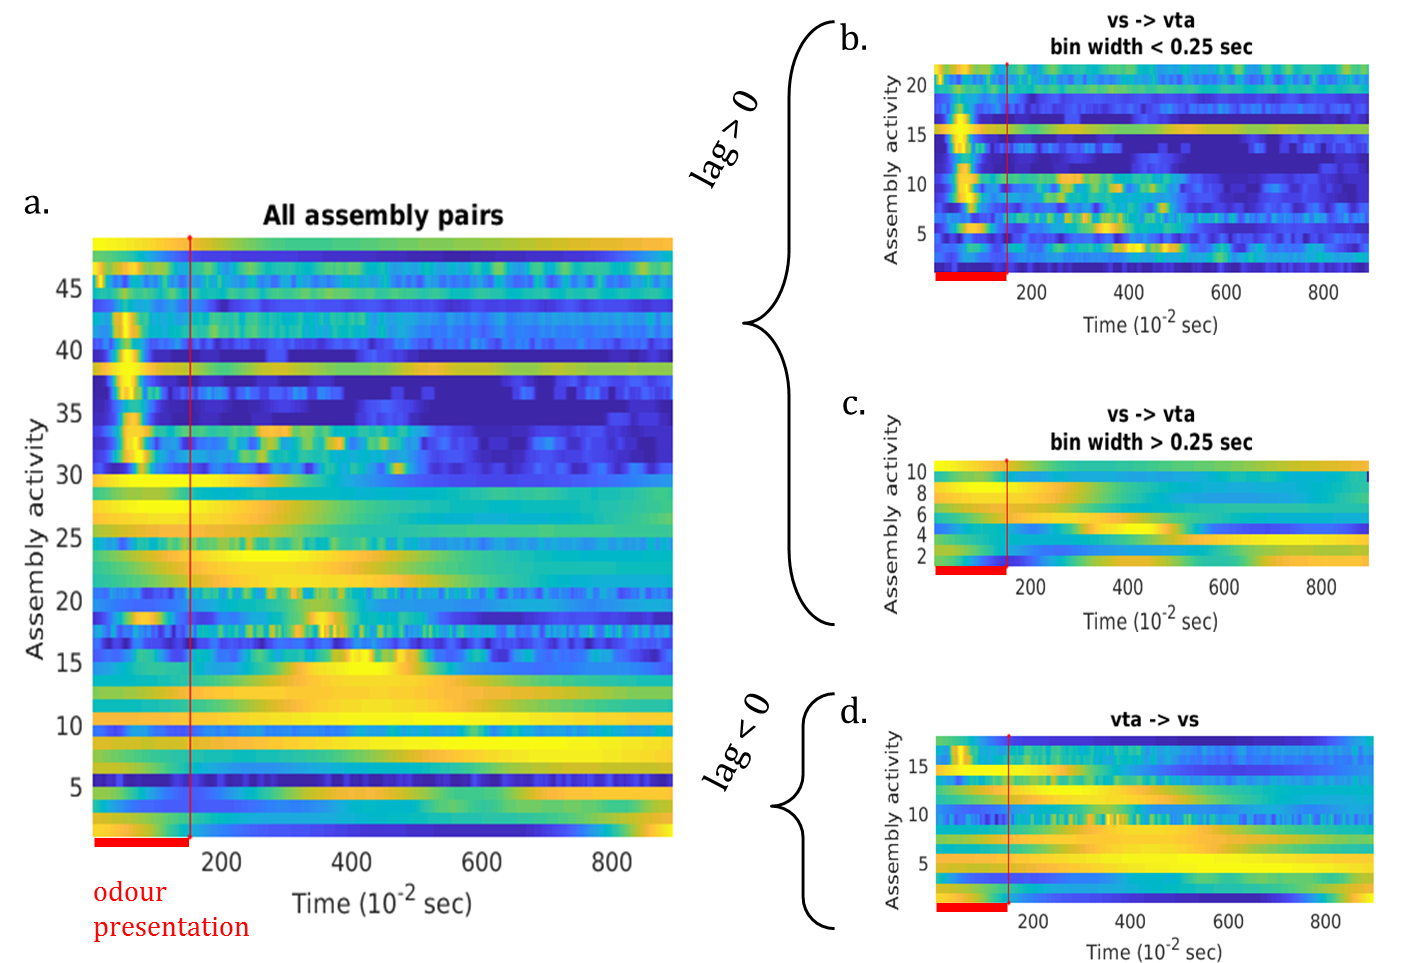
\includegraphics[scale=0.56]{figures/AsActPerBinLag1.png}
    \caption{Assembly-activation patterns given time bins and lags. In a. heat map of the activation of interregional pairs in one the experimental paradigms. The activation is normalized in such a way the activity range is $[0,1]$. Color scale ranges from deep blue, indicating the minimum possible, to yellow, indicating high activity. Pairs from a. were selected for bin size ($\Delta$) and lag: $\Delta < 0.25 s$ and $lag > 0$ (b.), $\Delta > 0.25 s$ and $lag > 0$ (c.), $lag < 0$ (d.)}
    \label{fig:AsActBinLag}
\end{figure}
%\begin{figure}[h!]
  %  \centering
  %%  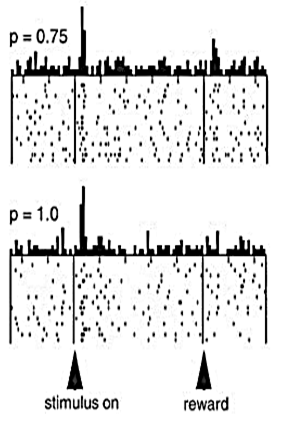
\includegraphics{figures/RewPred1.png}
   % \caption{Predictive reward signal in dopamine neurons. Adapted from \cite{Fiorillo}}
  %  \label{fig:RewPred}
%\end{figure}
%\pagebreak
\section{Conclusion}
From the interregional time scale distributions we deduced that VS-VTA assembly-pairs consisted in two classes of interactions with different time scales, highlighting the complexity of VS-VTA pair interactions and underling the importance of cell-assembly detection at different time scales.\\The two time scales involved in VS-VTA interaction were separated to study the lag analysis, revealing a preferred directionality $VS\rightarrow VTA$, and specifically in pairs containing striatal projection neurons and dopamine neurons.\\Different time scales of interaction and directionalities reflect different patterns of assembly-pair activity. Pairs detected at the precise time scale exhibited the directionality $VS\rightarrow VTA$ with a prominent activation during the stimulus presentation, as expected for prediction error signals.\\Since directional assemblies are formed by striatal projection neurons and dopamine neurons, we hypothesized that those pairs are good candidates for prediction coding. The next chapter is aimed to understand whether SPN-DAN assembly-pairs compute specifically prediction error signals. Comparing the activity of different assembly-pair types we therefore ask whether different assembly-pair types specialize in different coding features.\\

 \section{Pair-types task-related pattern}
 \label{sec:TaskResp}
In the previous section we concluded that time scale segregation and directionality might reflect specific task-related coding feature. In a data subset we have shown how different time scales and directionalities revealed different assembly-pairs activity patterns.\\We have seen as well that different assembly-pairs types have different directionality distribution. SPN-DAN assembly-pairs, in particular, exhibited a clear $VS\rightarrow VTA$ directionality, so we expect those assembly to have different patterns of activity with respect to other assembly-pair types.\\Furthermore in this section we will test whether different assembly-pairs-types have different task-related activity patterns, and consequently express different coding functions.\\
To this purpose, we tested the responsiveness of each assembly-pair to the conditioned stimulus (CS $+/-$) and the unconditioned stimulus (US), through an analysis of variance performed using both a paired Friedman test and a non parametric version of repeated measures ANOVA test, on the basis of trial by trial assembly-pair activity. The results of the two tests were consistent each other. We choose to present here only Friedman test results, as it is free from gaussianity assumptions.\\Time intervals were 0.5 $sec$ long, and were chosen as follows: CS $+/-$ interval included all time steps $t \in [0, 0.5]$ $sec$ from the odor onset, CS$+/-$cont. was the window including each time $t$ with $t \in [-0.5, 0]$ $sec$ before the reward retrieval, in which the the odor was still present, US interval included times $t \in [0,0.5]$ from the reward delivery. The assembly-pair activity in the listed task relevant intervals was compared with the baseline interval including times $t \in [-0.8, -0.3]$ $sec$ before the odor onset, in which task related activity should be low.\\For each assembly-pair type we performed a large number of statistical tests, some will have p-values less than $0.05$ purely by chance, even if all null hypotheses of the family of tests performed are really true. Hence, Bonferroni correction for multiple comparison was applied. The Bonferroni correction is the classical approach to take in account the multiple comparison problem and consists in having a control on the familywise error rate ($\alpha=0.05$). This is possible by setting the critical value $\alpha$ for an individual test at lower value than 0.05 in such a way that, if all the null hypotheses are true, the probability that the family of tests includes one or more false positives due to chance is 0.05. The value $\alpha$ for an individual test is obtained by dividing the familywise error rate by the number of tests.\\Figure \ref{fig:Baseline} shows the heat map of the neural activity averaged across trials before and after the odor onset, during the baseline period (interval delimited by the two back lines) no activity patterns emerge besides the spontaneous neural activity.\\
\begin{figure}
    \centering
    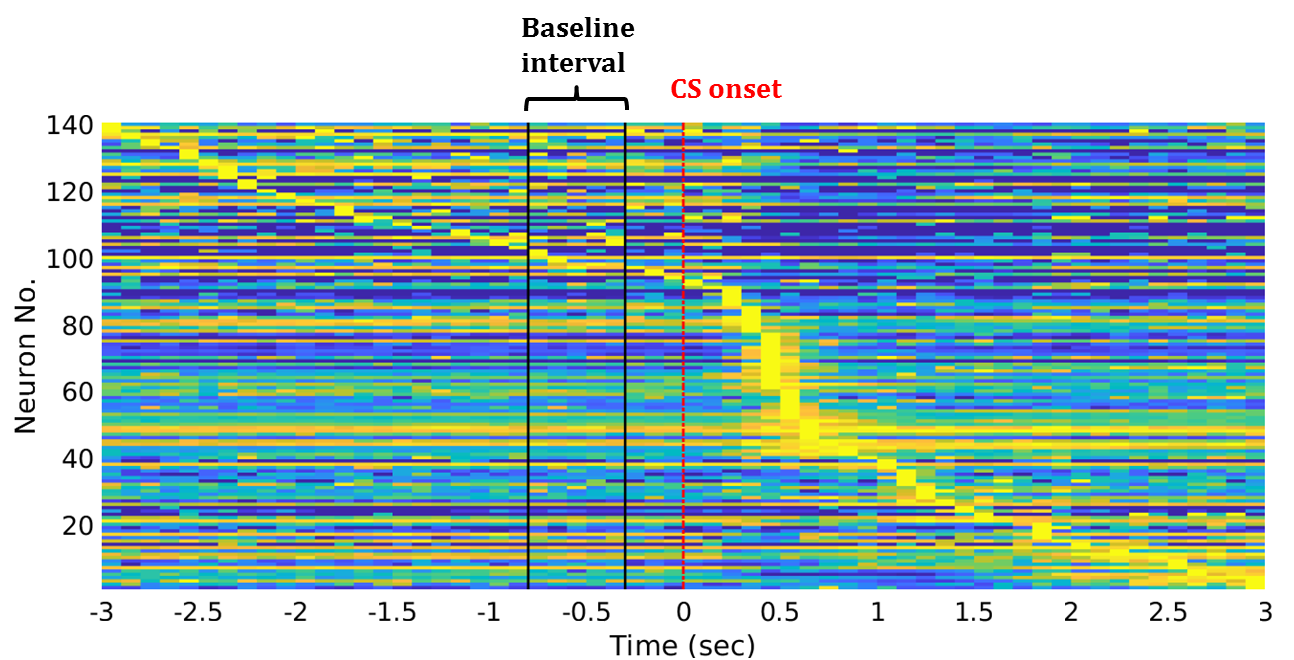
\includegraphics[scale=0.6]{figures/Baseline.png}
    \caption{Baseline interval choice. Neural activity averaged across trials. For each trial the baseline interval was a time window in which no task related activity could have interfered with the spontaneous neural activity. Again color map ranges from blue to yellow indicated with blue the minimum of activity and in yellow the maximum.}
    \label{fig:Baseline}
\end{figure}
Analysis of variance compares the means of several groups to test the hypothesis that they are all equal, against the general alternative that they are not all equal. This alternative was in our case too general. Hence, in the cases in which we obtained an omnibus significant $\chi^2$ test, the post-hoc procedure were designed using the matlab function $\textit{multcompare}$ whose critical values where computed with Bonferroni method (\cite{Bonferroni}, \cite{Dunn1958}, \cite{Dunn1961}).\\
\begin{figure}
    \centering
   % 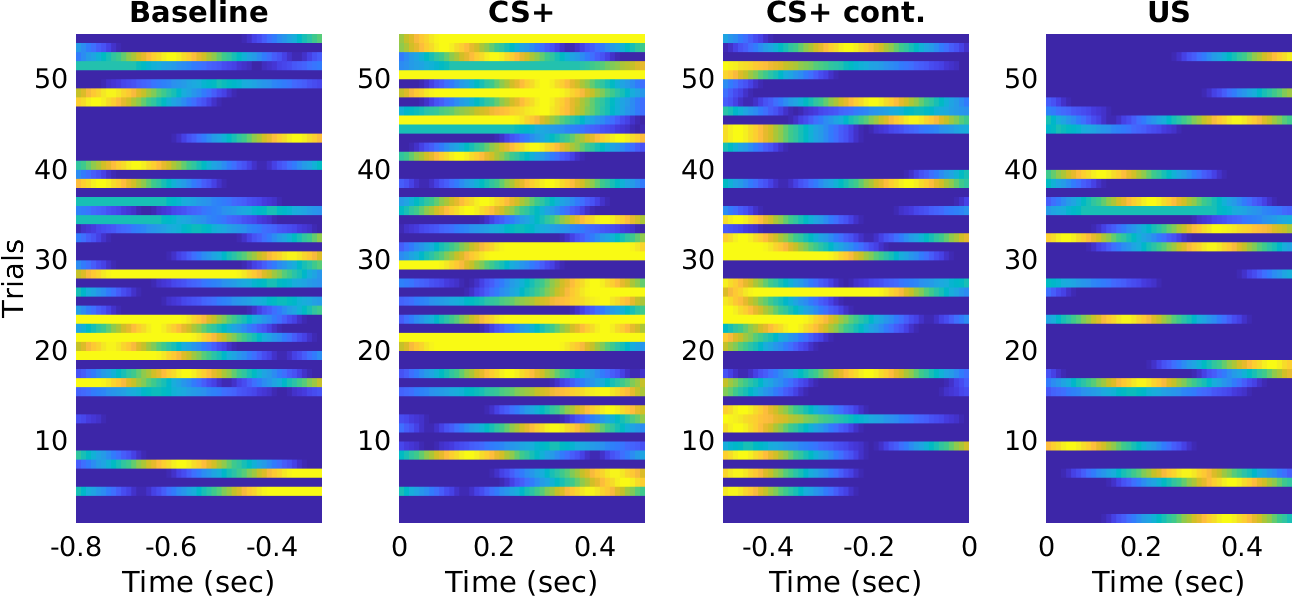
\includegraphics[scale=0.4]{figures/SPN_DANexStim1.png}
    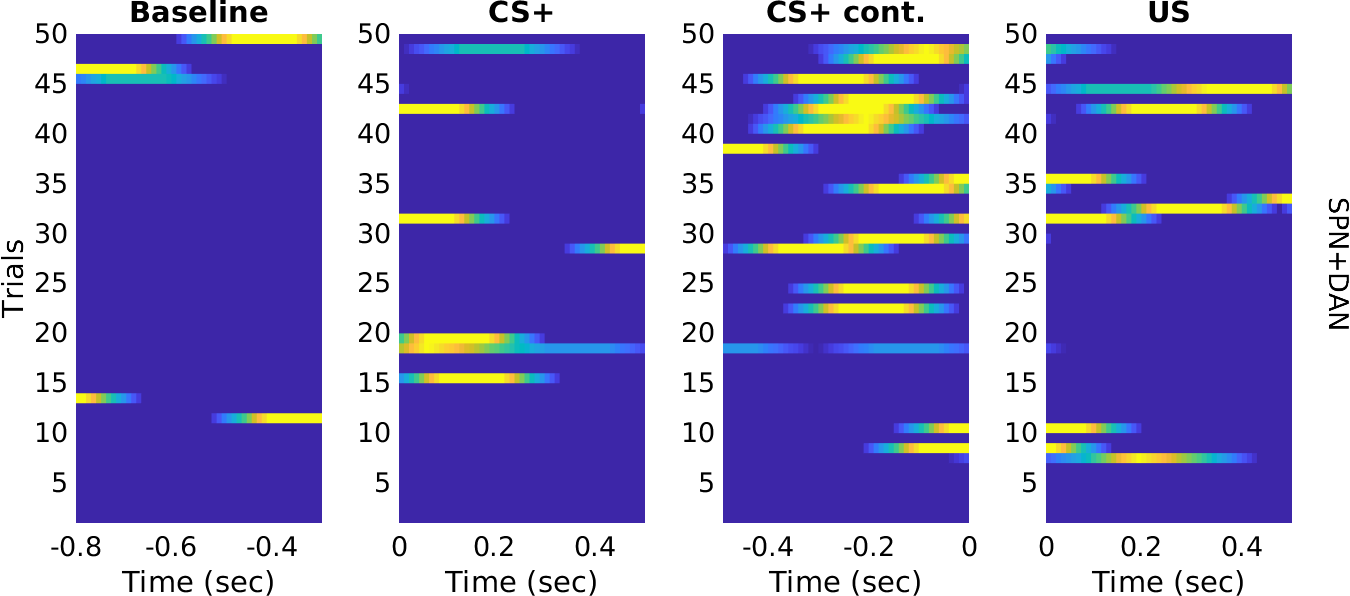
\includegraphics[scale=0.38]{figures/SPN_DANexPreRew.png}
    
   \vspace{1cm}
   
   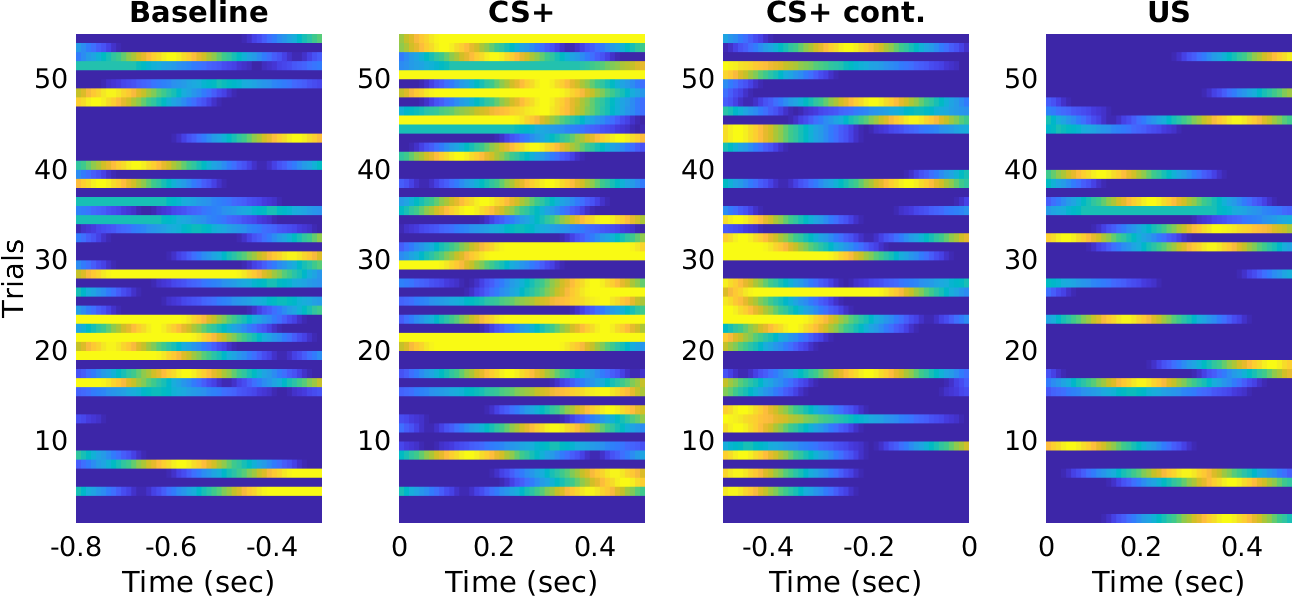
\includegraphics[scale=0.38]{figures/SPN_DANexStim1.png}
    \caption{Example of two assembly-pairs significant after the analysis of variance for which the post-hoc test shown that in both cases two groups out of four were significant different, respectively the baseline and the CS+$_{cont}$ window (top) and the baseline and the CS+ window (bottom).}
    \label{fig:SPN_Ex}
\end{figure}
In figure \ref{fig:SPN_Ex}, two examples of assembly-pairs were significant for the Friedman test performed on hit trials (correct trials when the rewarded odor was presented).\\We examined two SPN-DAN pairs closer that had significant difference between the baseline and the CS+$_{cont.}$ groups (\ref{fig:SPN_Ex}, top) or the baseline and CS+ (\ref{fig:SPN_Ex}, bottom) groups. Interestingly we observed, in significant windows, less assembly-activity in the first trials and intense assembly-activity in the last trials.\\This dynamical responsiveness resembles typical learning dynamics. In first the trials the mouse is in an explorative period in which the rule of the task has not been learnt yet; while it has been learnt at the end of the original phase. In other words, in the first part of the task the animal is almost always surprised when the reward is delivered, the expectation of reward is low, while during the second part of the original phase the mouse is able to predict the reward already at the stimulus presentation, the expectation of reward increases when the rewarded stimulus is presented.\\In presence of probabilistic reward the response of dopamine units is peaked at the reward time when the probability to get the reward is low and is instead peaked at stimulus presentation when the probability to get the reward is high (\cite{Schultz1992}, \cite{Schultz} \cite{Fiorillo}). VS neurons instead show a tonic response with the stimulus presentation and their neuronal activity is modified when the subject learns to predict future rewards from sensory cues (\cite{Pagnoni}, \cite{Schultz2000}, \cite{Radua}).\\Thus if an assembly-pair codes for reward prediction error, then the activity should be intense during the presentation of the rewarded stimulus only in the last part of the task-phase. On the contrary in pairs significant at retrieval (US) we would expect intense activity in first trials, related to the surprise to have the reward, and less activation in the second part of task, when the animal acquired sureness about the reward. We will examine these learning transitions revealed in the variability across trials in\hyperref[sec:CorrRL]{~Chapter \ref*{sec:CorrRL}}.\\
The two examples in figure \ref{fig:SPN_Ex} above show that some assembly-pairs are implicated in the learning dynamic, with a systematic study in this direction we can understand how many of them are involved in the learning dynamic and which functions they express. Assuming that a good portion of assembly-pairs show a learning dynamic, we ask: are they all involved specifically in prediction error computation? Do they compute differently the prediction error signal depending on their underlying units? Reward prediction error signal in DAN is formed by two components (\cite{Tobler2003}, \cite{Nomoto2010}, \cite{Fiorillo2013}, \cite{Schultz2016}): the first component consists in an early activation due to an unselective response to a large variety of unpredicted events included the potentially rewarded stimuli, that are however in this phase only detected, to be later identified and valuated.\\The detection component evolves then into the second component, also called main component, which reflects the evolving neuronal processing that is required to fully appreciate the value of the stimulus (see figure \ref{fig:probSchultz} in\hyperref[sec:StateArt]{~Chapter \ref*{sec:StateArt}}). The latter component is the biological implementations of reward prediction error term in reinforcement learning models.\\DAN express both these two components, showing homogeneity in response in order to ensure a robust and efficient coding \cite{UchidaDop}. Despite clear evidence for DAN involvement in prediction coding, it is hard to identify how these signals are encoded by the larger circuit. In this work we want to prove that the specificity of different components coding emerges in the assembly-pairs activity because different interactions convey different aspects of the prediction error coding. Thus DAN exhibit homogeneous but robust responses at population level, which could become specific through distinct VS interactions. The learning functions would be then, rather than cell-types-specific, circuit specific (\cite{Saunders2018}).\\
We start to prove this hypothesis by analysing the reward-related activity of assembly-pair types.\\
We focused the analysis on assemblies resulting significant for the Friedman test, the fraction in percentage of those assemblies is shown in figure \ref{fig:PercAsFried}. The histograms refer to the Friedman tests made on hit trials, in original and reversal phase separately.\\
\begin{figure}
    \centering
    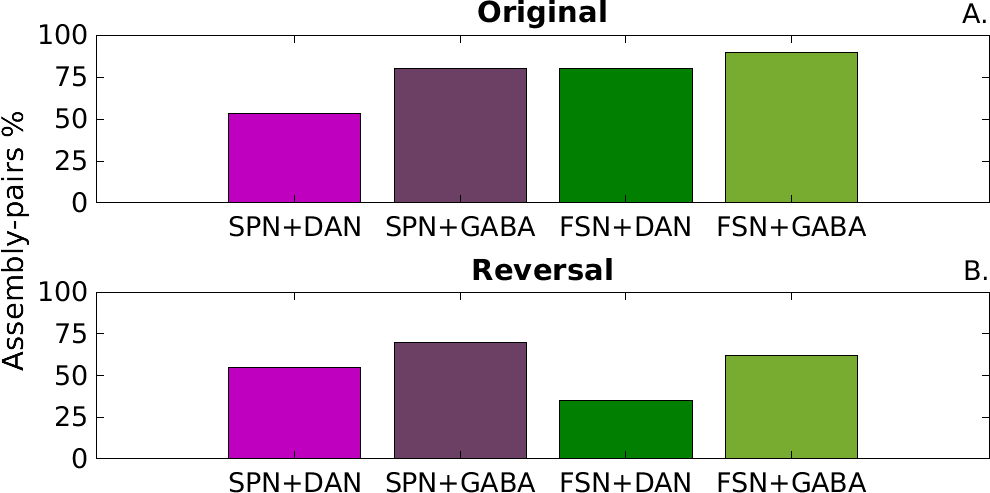
\includegraphics[scale=0.5]{figures/PercFriedHitTrialsBFf.png}
    \caption{Number in percentage of assembly-pairs exhibiting a significant task related pattern activity. The Bonferroni correction for multiple comparison was applied. In A. the significant assembly-pairs tested for the original phase, in B. the significant assembly-pairs tested in reversal. Assembly are divided in the four principal pair-types.}
    \label{fig:PercAsFried}
\end{figure}
Assembly-pairs patterns of significant assemblies were plotted, and differences in assembly-types emerged. Figure \ref{fig:HeatPairsDan} shows assembly-pairs tested with Friedman test and resulting to have significant task related response in original phase. In order: A1. SPN-DAN assembly-pairs in original phase: a good portion of those pairs became active early at the rewarded stimulus (CS+) presentation, a good portion remained active during the stimulus presentation (CS+$_{cont.}$). Only a small fraction was active only in US window. SPN-DAN assembly-pairs are thus good candidates for prediction coding. In A.2 the same assembly-pairs in the reversal phase.\\FSN-DAN assembly-pairs on contrast have a phasic early response to the rewarded stimulus (CS+) or reward retrieval (US) (B.1); in B.2 same FSN-DAN pairs in the reversal phase, with respect to the original phase we notice less activation at the stimulus onset (CS+) and more at US.\\The early activation to the stimulus of FSN-DAN pairs may suggest that they are involved in the detection coding. One hypothesis could be that the detection component of prediction error is formed in FSN-DAN assembly-pairs, which evolves in the identification and valuation coding through the SPN-DAN circuit. Those consideration will be discussed in detail in \hyperref[sec:FalseAlCorrRej]{Section~\ref*{sec:FalseAlCorrRej}}, as well in \hyperref[sec:CorrRL]{Chapter~\ref*{sec:CorrRL}}, and \hyperref[sec:Regression]{Chapter~\ref*{sec:Regression}}.\\In figure \ref{fig:HeatPairsDan} and figure \ref{fig:HeatPairsGaba} we see that different assembly-types are active in different task moments, summary plots are shown in figure  \ref{fig:FriedHistoDAN} and figure \ref{fig:FriedHistoGABA} where we report in which windows (CS+, CS+$_{cont.}$, US) assembly-pairs are significantly active with respect to the baseline. The total amount can exceed the $100\%$, for example, if one pair was found significant in the US window and CS+$_{cont.}$ with respect to the baseline, this assembly-pair was double counted.\\All assembly-pair types are predominantly active in the window CS+$_{cont.}$, that is the window of preparation for the retrieval.\\There were differences among assembly-pairs types and phases. The first remarkable difference is between the original and reversal phase: in the reversal phase all pair-types were less activated in CS+ window with respect to the original phase. In assembly-pairs including SPN the decrease in activity in CS+ corresponded to more activity at retrieval (US) in the reversal phase, reflecting the reward-related surprise, expected to be more accentuated in reversal phase. Assembly-pairs composed by GABA units became activated later than assembly-pairs composed by DAN, and they are broadly active before the reward and during the reward consumption. Pairs with GABA or DAN were predicted to encode different signals, and indeed showed different task related patterns.\\Since we specifically want to investigate how prediction signals are formed in VS-VTA interaction, we focused only on the interregional assembly-pairs with DAN in the subsequent analysis.\\
 \begin{figure}
     \centering
     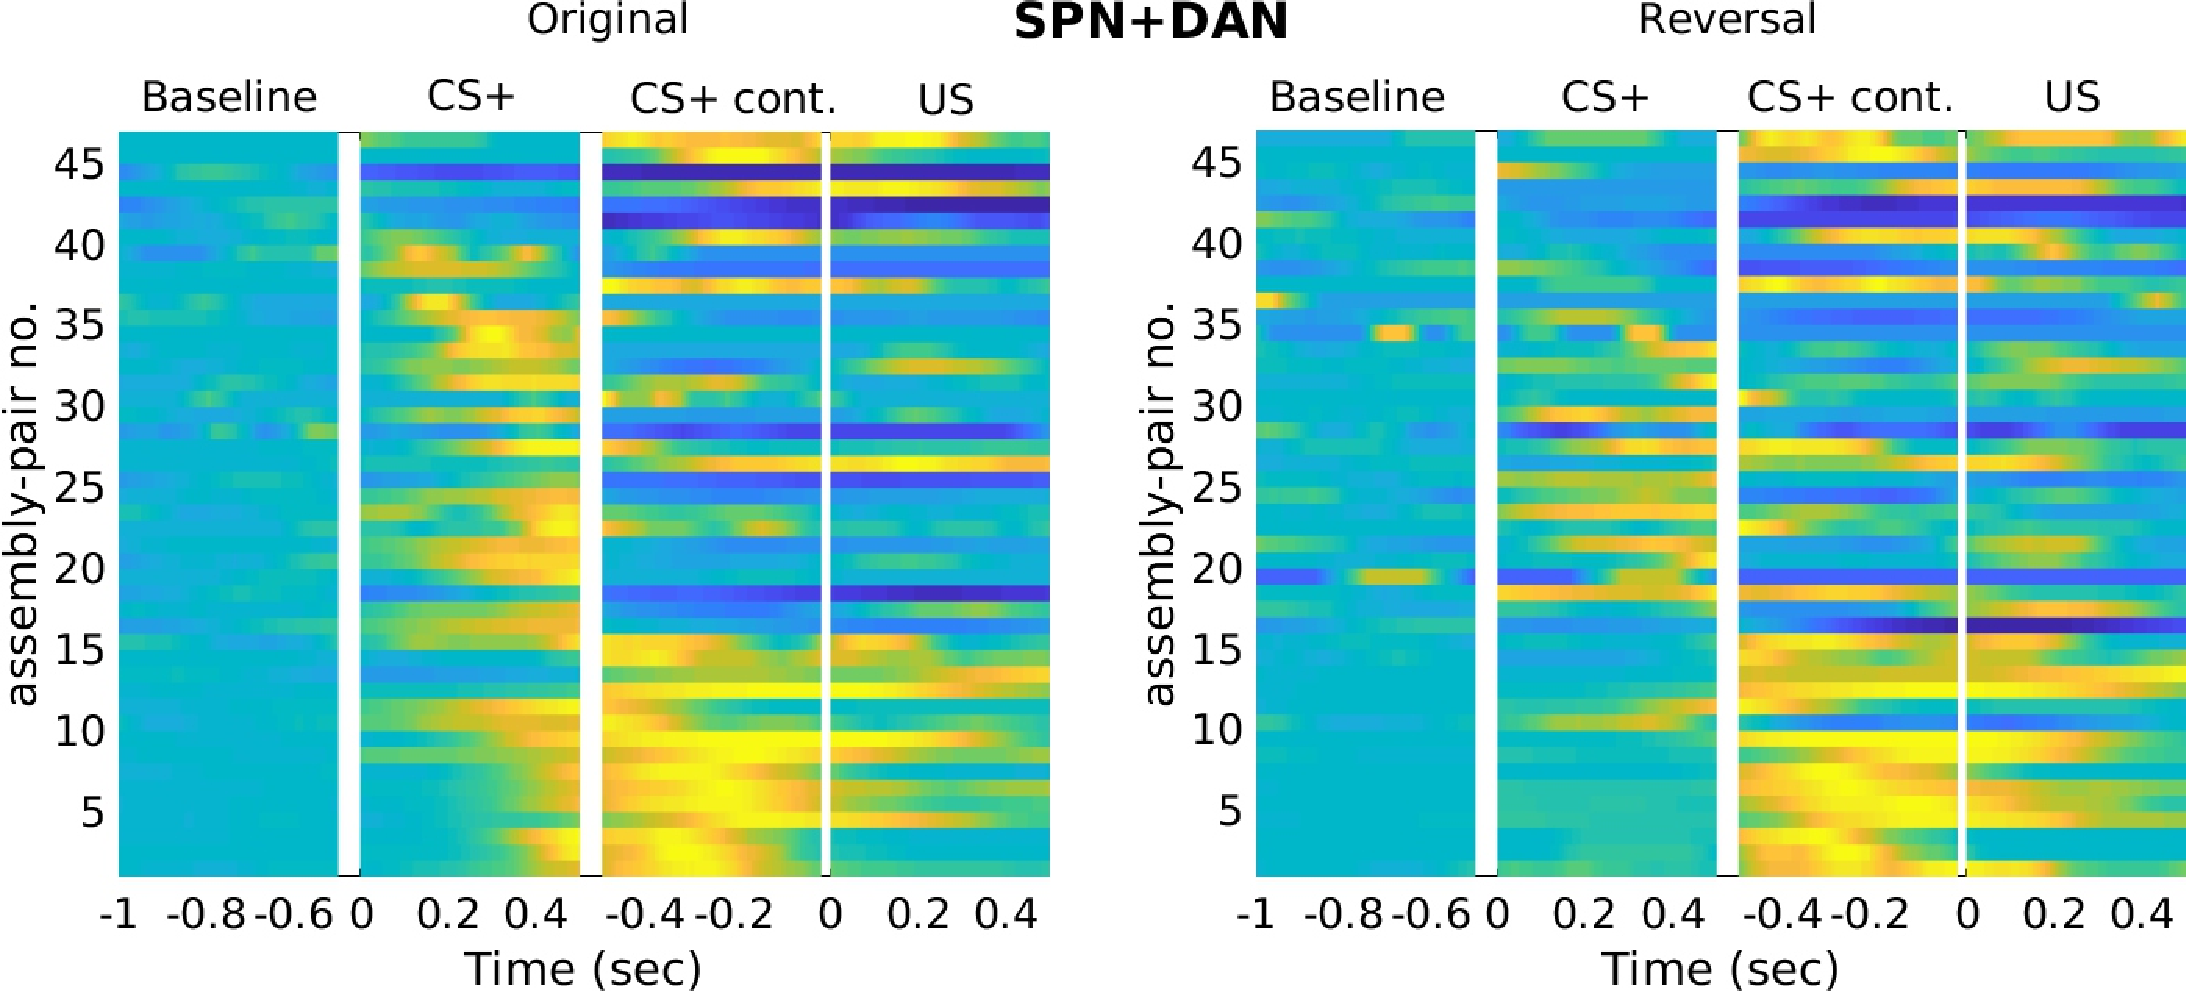
\includegraphics[scale=0.32]{figures/SPN_DAN.pdf}
     
     \vspace{1cm}
     
     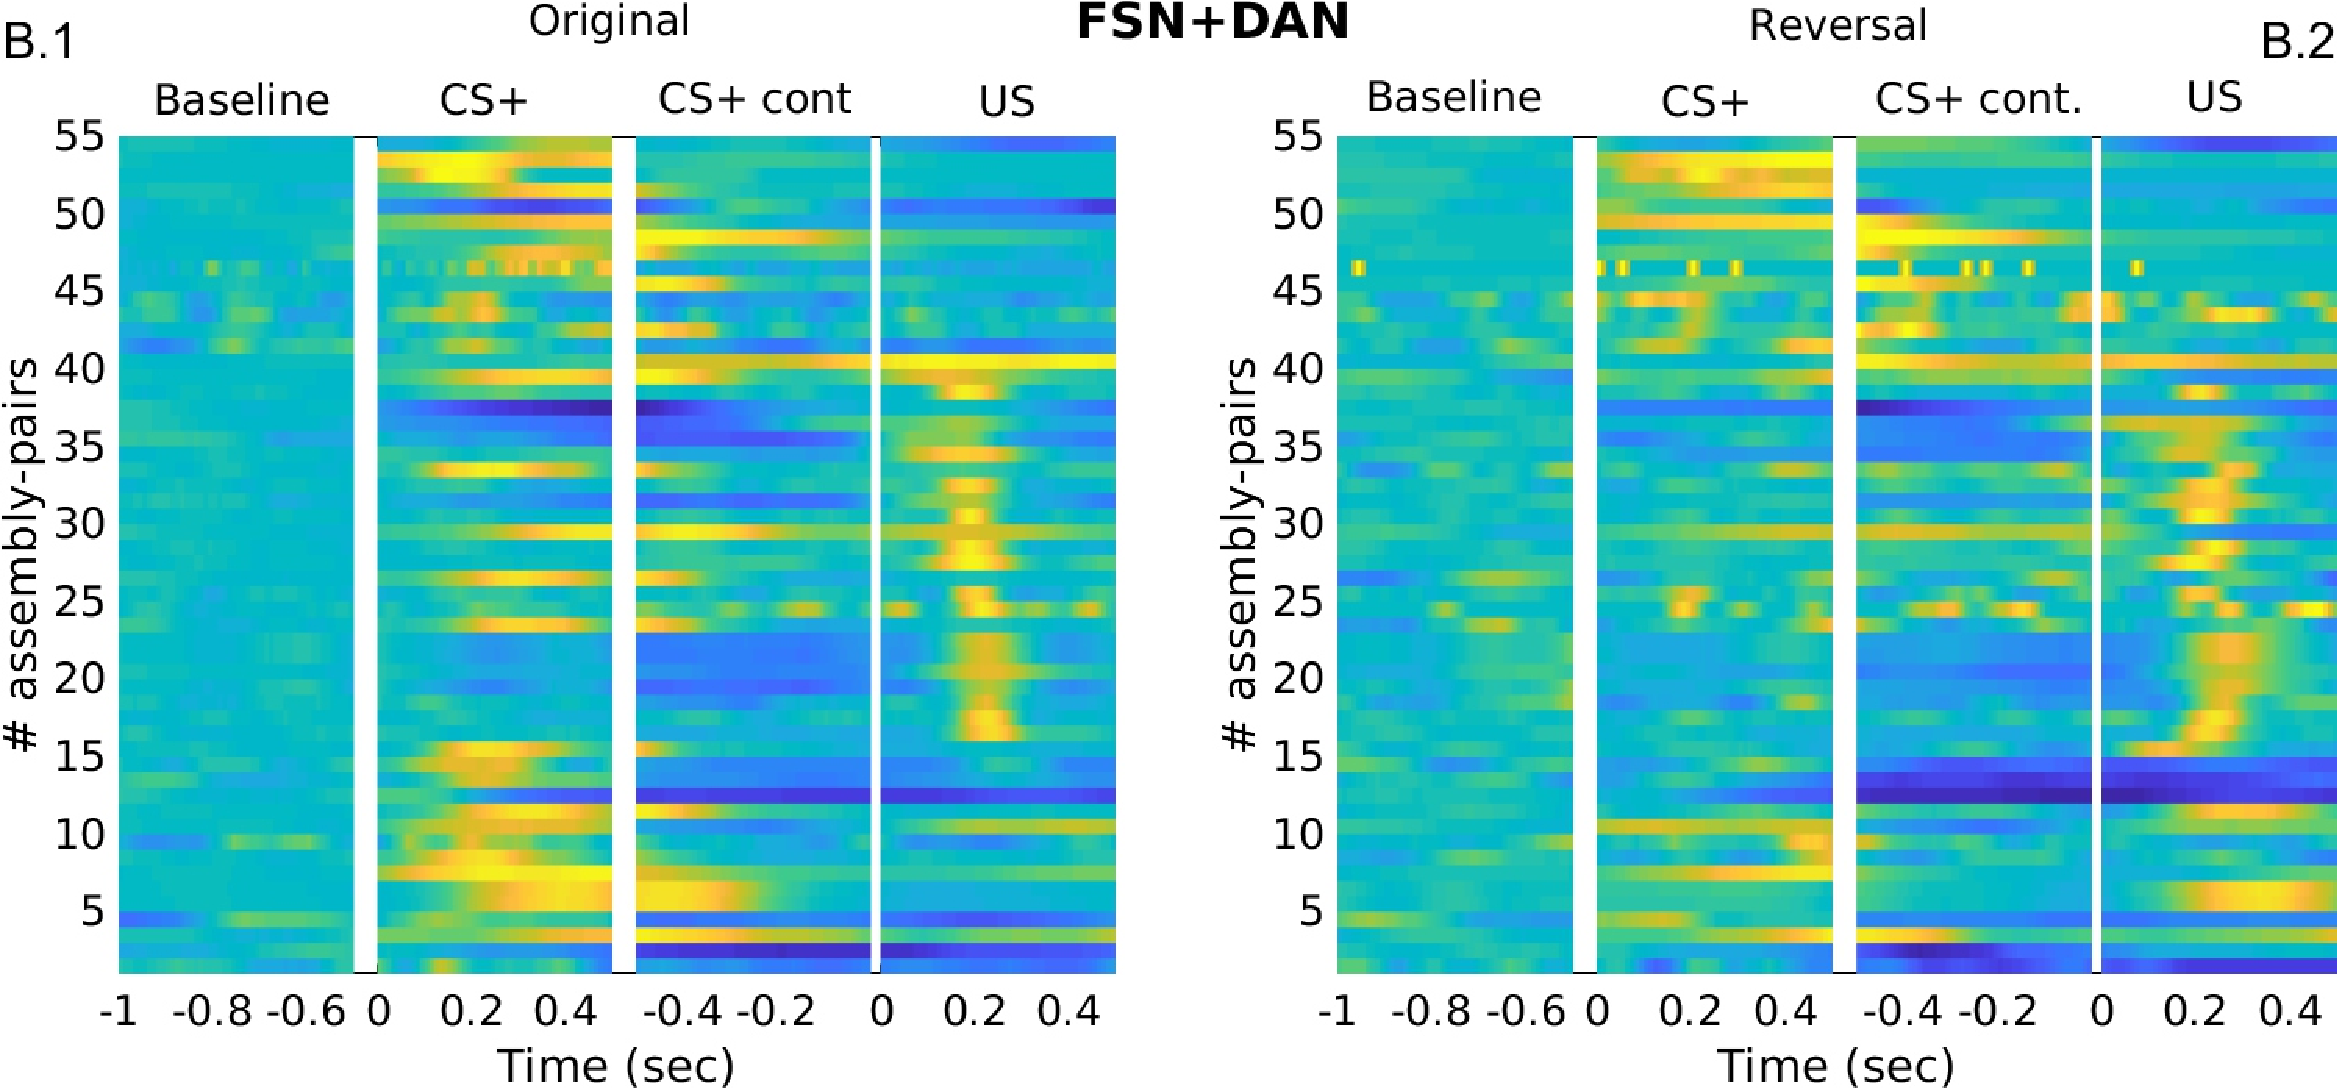
\includegraphics[scale=0.32]{figures/HeatFSN_DAN.pdf}
     \caption{Assembly-pairs tested with Friedman test with significant task related response in original phase. In order: \textbf{Top left:} SPN-DAN assembly-pairs; \textbf{top right:} the same assembly-pairs in the reversal phase. \textbf{Bottom left:} FSN-DAN assembly-pairs; \textbf{bottom right:} same FSN-DAN pairs in the reversal phase. The color map ranges from blue to yellow, indicating in deep blue inhibition, in turquoise almost no activation and in yellow high activation. The activity of each assembly was normalized as in eq.\ref{eq:norm} were $\max(I)$ ($\min(I)$) was the absolute maximum (minimum) of assembly-activity among the four windows.}
     \label{fig:HeatPairsDan}
 \end{figure}
 \begin{figure}
     \centering
     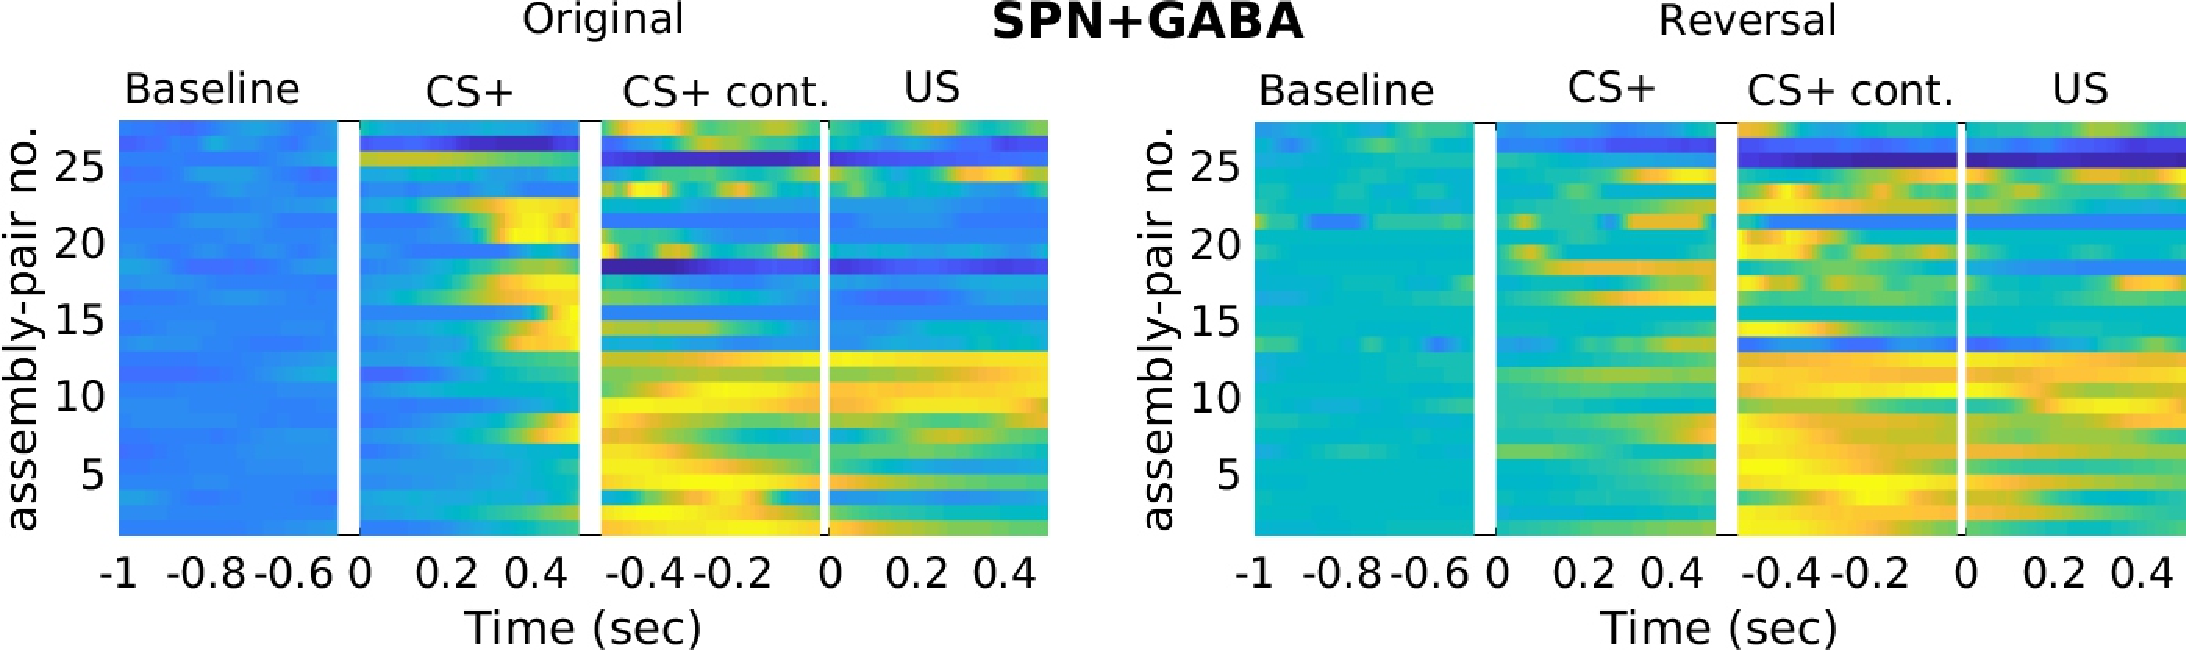
\includegraphics[scale=0.32]{figures/HeatSPN_GABA.pdf}
     
     \vspace{1cm}
     
     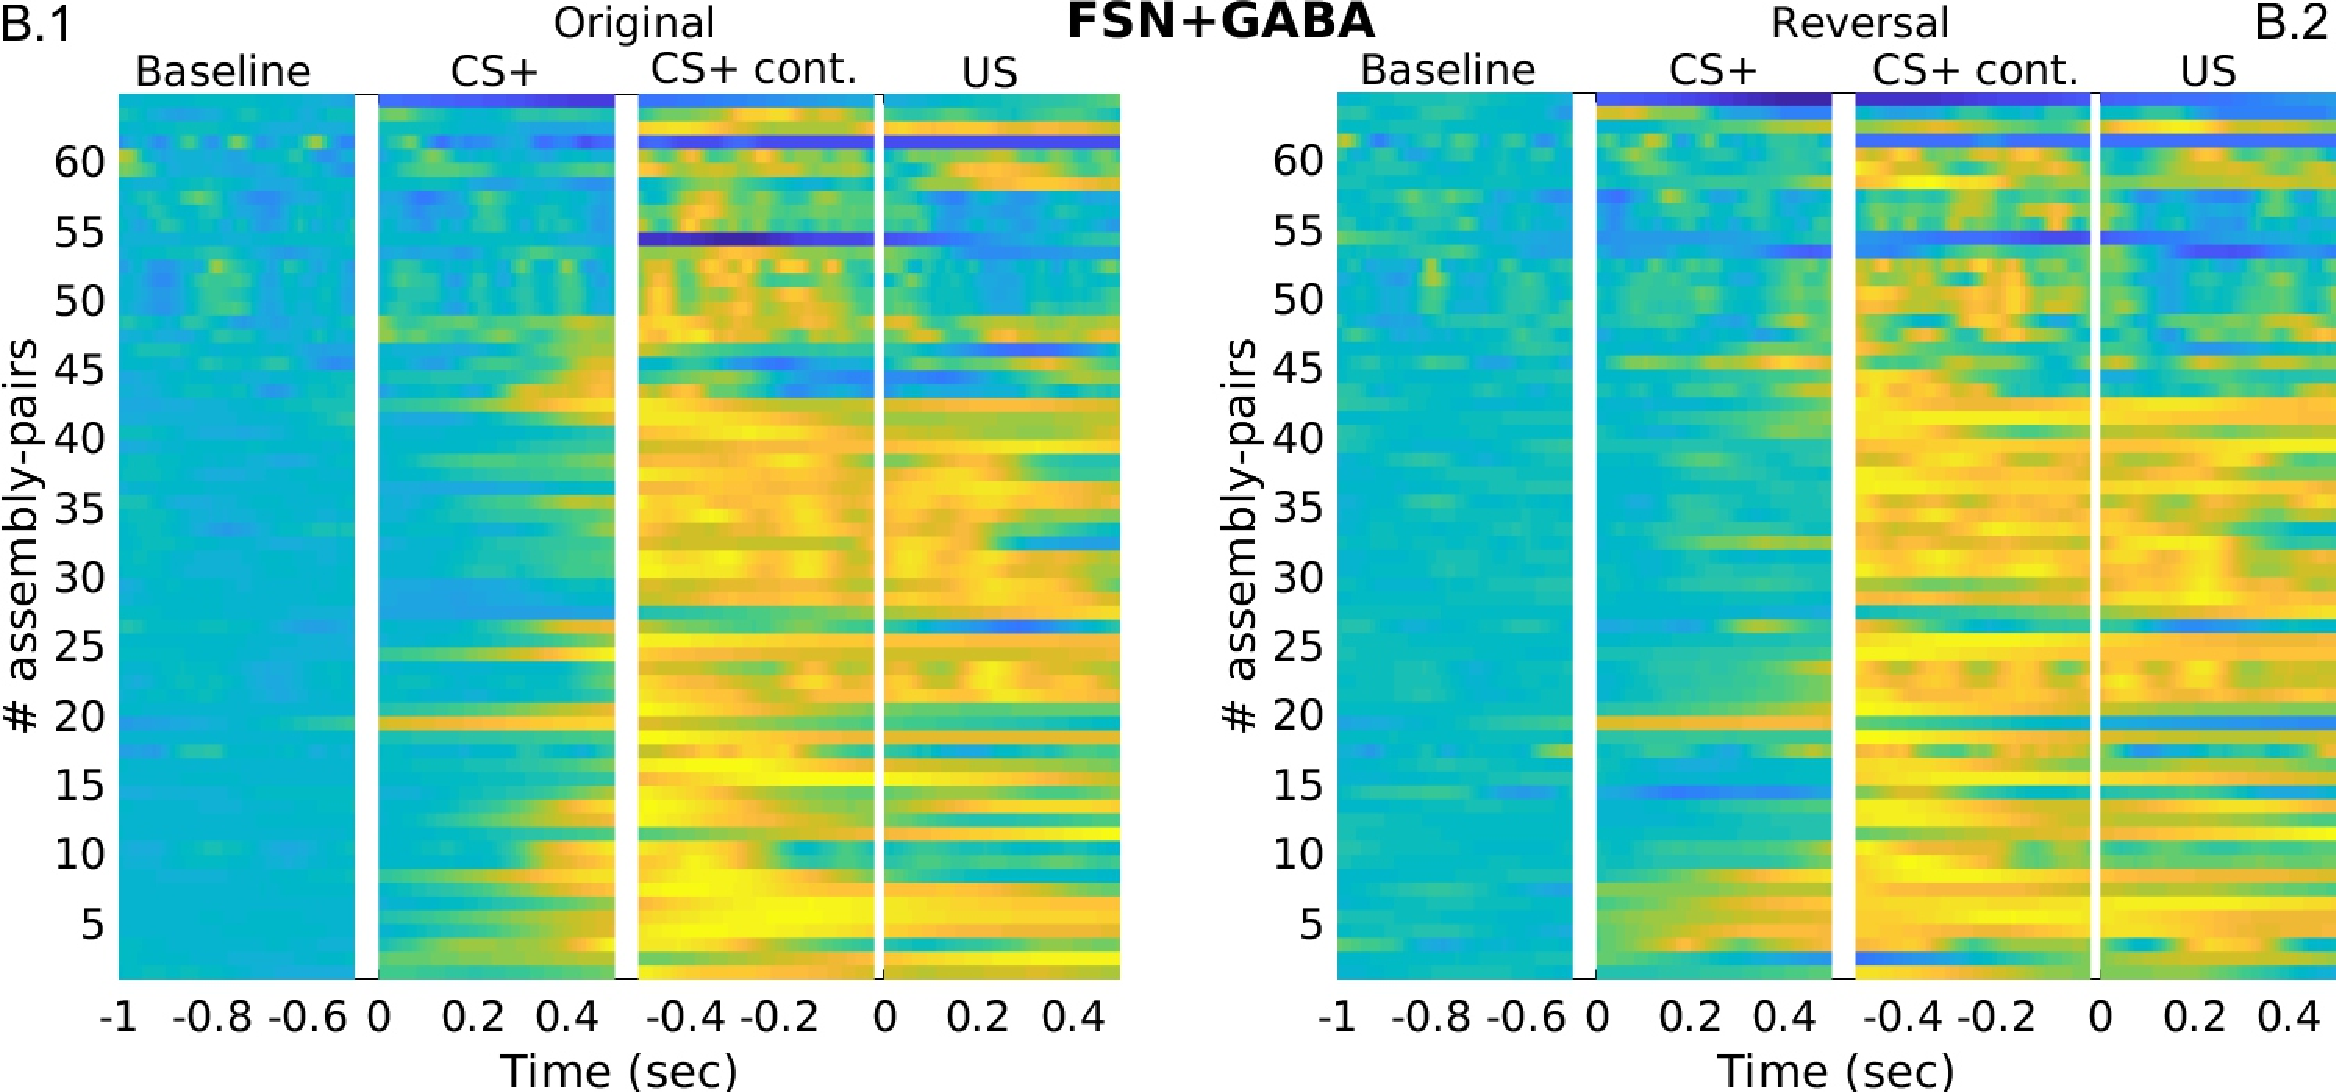
\includegraphics[scale=0.32]{figures/HeatFSN_GABA.pdf}
     \caption{Assembly-pairs tested with Friedman test with significant task related response in original phase. In order: \textbf{Top left:}SPN-GABA assembly-pairs; \textbf{top right:} the same assembly-pairs in the reversal phase. \textbf{Bottom left:} FSN-GABA assembly-pairs in original; \textbf{bottom right:} FSN-GABA assembly-pairs in reversal. The color map ranges from blue to yellow, indicating in deep blue inhibition, in turquoise almost no activation and in yellow high activation. The activity of each assembly was normalized as in eq.\ref{eq:norm} were $\max(I)$ ($\min(I)$) was the absolute maximum (minimum) of assembly-activity among the four windows.}
     \label{fig:HeatPairsGaba}
 \end{figure}
 \begin{figure}
    \centering
    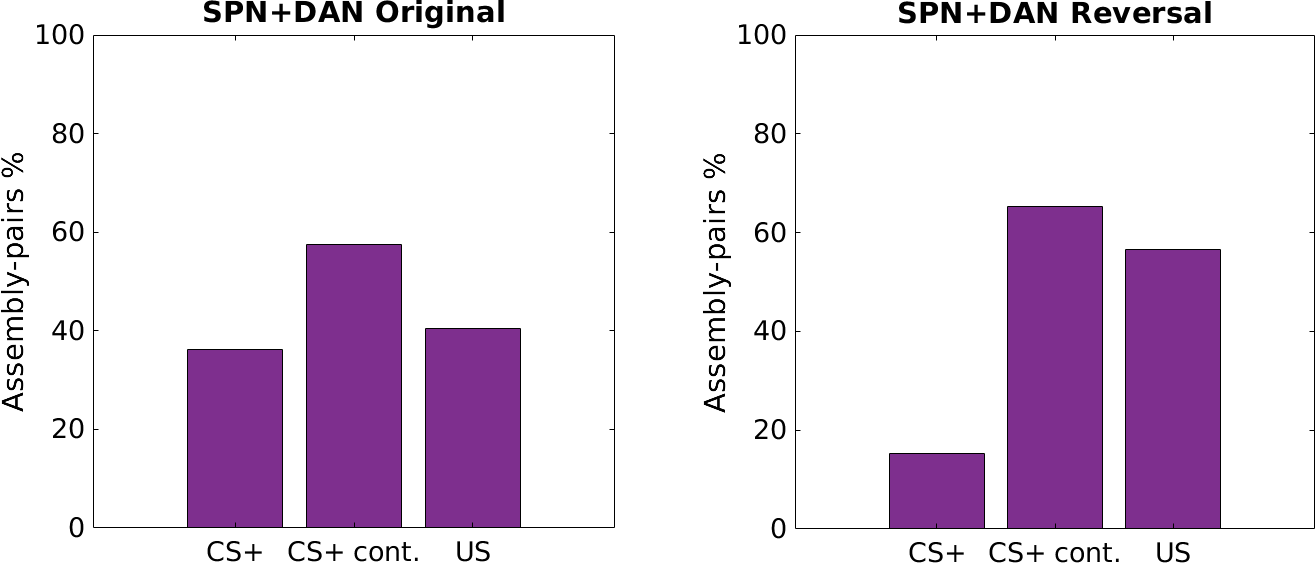
\includegraphics[scale=0.36]{figures/SPN_DANHisto.png}
    
    \vspace{1cm}
    
    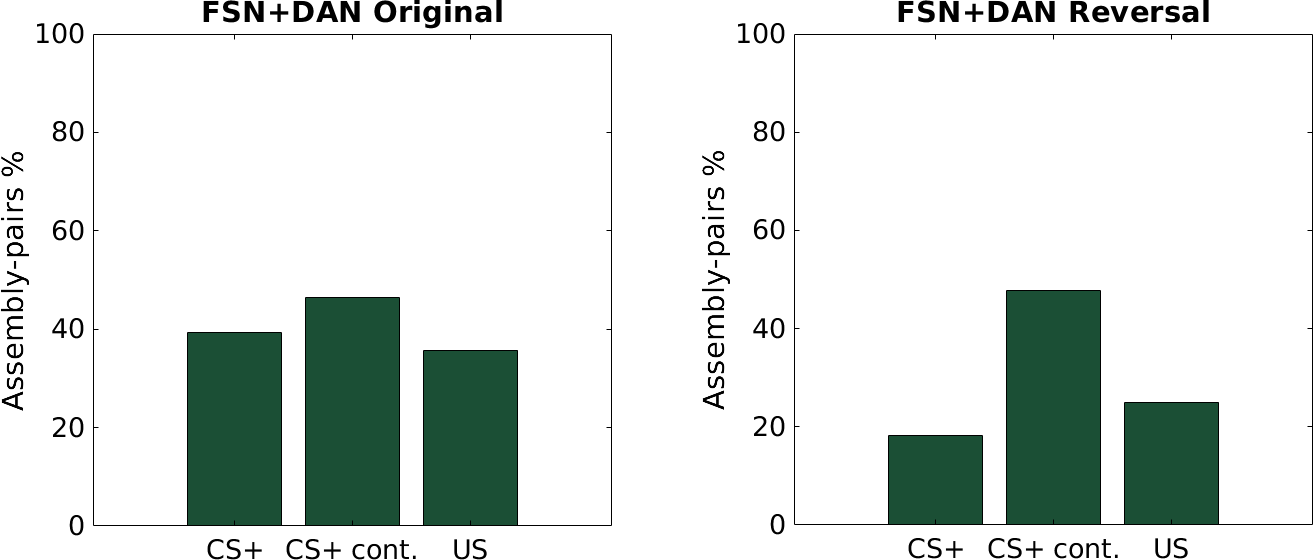
\includegraphics[scale=0.36]{figures/FSN_DANHisto.png}
\caption{Percentage of assembly-pairs significant with respect to the baseline in the windows CS+, CS+$_{cont.}$, US. The total amount can exceed the $100\%$ because if  one pair were found for example significant in the US window and CS+$_{cont.}$ with respect to the baseline, this assembly-pair was double counted.}
    \label{fig:FriedHistoDAN}
\end{figure}
\begin{figure}
    \centering
    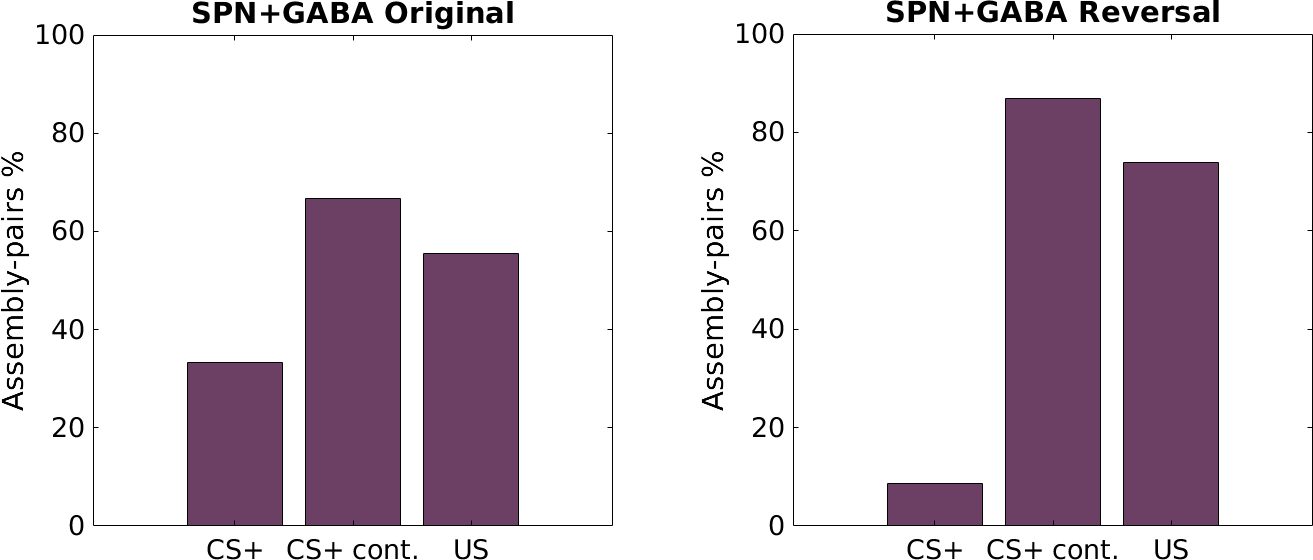
\includegraphics[scale=0.36]{figures/SPN_GABAHisto.png}
    
    \vspace{1cm}
    
    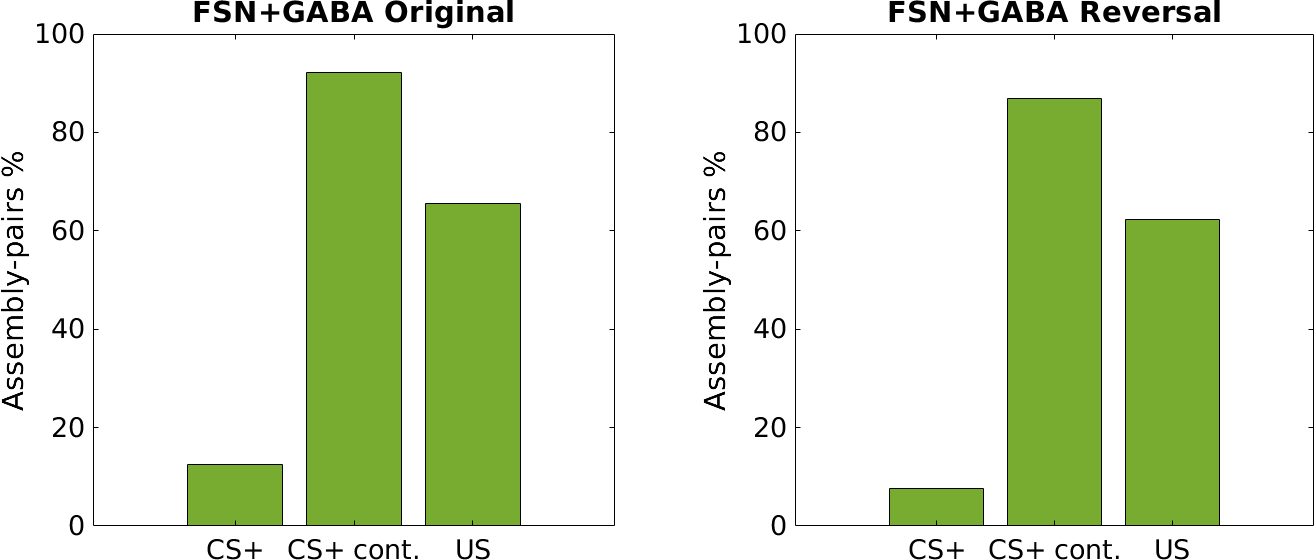
\includegraphics[scale=0.36]{figures/FSN_GABAHisto.png}
    \caption{Percentage of assembly-pairs significant with respect to the baseline in the windows CS+, CS+$_{cont.}$, US. The total amount can exceed the $100\%$ because if one pair were found for example significant in the US window and CS+$_{cont.}$ with respect to the baseline, this assembly-pair was double counted.}
    \label{fig:FriedHistoGABA}
\end{figure}\\
\pagebreak
\section{Hit, False Alarm and Correct Rejection Trials}
\label{sec:FalseAlCorrRej}
When the animal receives reward unexpectedly, DAN fire a burst of action potentials. If a sensory stimulus reliably predicts reward, however, DAN decrease their response to reward, and instead burst to the stimulus, and finally if an expected reward is omitted, DAN pause their firing at the time they usually receive reward (\cite{Schultz1997}, \cite{Wenzel}, \cite{Fiorillo2013b}, \cite{Schultz2015}).\\The comparison between Hit, False Alarm and Correct Rejection is interesting because we expect different VS-VTA assembly-pair activations in relation with reward prediction and reward occurrence.\\We assumed that assembly-pair task related patterns reflect the predictive coding of underlying units, furthermore we expected that assembly analysis could reveal how the prediction signal is formed in VS-VTA circuit, question that is in fact still discussed and unclear (\cite{Takahashi2016}, \cite{Saunders2018}).\\If our hypothesis of a circuit specialized code is true, we should observe differences in activity patterns of VS-VTA assembly-pairs composed by DAN with different cell-types in VS. In the previous session we introduced the two sequential components of neuronal response, the first called detection, and the main component, called identification and valuation. We suggested as well that sharp assembly-pairs FSN-DAN most probably encode a generic detection of the stimulus, whereas SPN-DAN assembly pairs, characterized by broader response could encode the valuation, that is the component associated to the prediction error in reinforcement learning models.\\ In the previous section we examined related response of assembly-pairs in Hit trials, namely trials in which the odor was followed by reward and the mouse went for the reward. We had identified, in specific moments of the trial, assembly-pairs with significant task-related activation.\\In the same way, we had analysed the assembly-pairs task-related response for False Alarm trials (unrewarded odor, the mouse went for reward) and Correct Rejection trials (unrewarded odor, the mouse sat quiet). The three windows of interest were set up for these trials types in the following ways: in False Alarm trials those windows were called CS-, CS-$_{cont.}$, 3rd Lick. The CS- window, analogously to the CS+ in Hit trials, was a time interval of 0.5 $sec$ starting from the stimulus onset (unrewarded in this case); the CS-$_{cont.}$ and 3rd Lick were respectively the time intervals, again 0.5 $sec$ long, immediately before and after the expected reward.\\We used the following assumption to establish the expected reward time: in the cases in which the rewarded odor was presented the mouse had to lick at least two or three times (depending on the paradigm) to get the reward, thus when it licked despite the odor was unrewarded, it was considered to expect the reward after the second or the third lick (depending on the current paradigm).\\In Correct Rejection trials, CS- and CS-$_{cont.}$ intervals were defined similar to the False Alarm trials. In this case the animal did not expect the reward, however, we analysed the assembly-pairs activity also in the $"$hypothetical reward$"$ window for comparison. We used as $"$hypothetical reward$"$ time, the average reward time obtained from Hit trials, to compare the assembly-pairs activity before and after the $"$hypothetical reward$"$ time with the activity before and after the reward time (Hit trials) or the expected reward time (False Alarm trials).\\
\subsection{SPN-DAN assembly-pairs}
Figure \ref{fig:HeatSPN_DANComp} shows SPN-DAN pairs task-related activity in Hit, False Alarm and Correct Rejection trials. In Hit trials the assembly-pairs activation was lead mainly by the rewarded odor. A good portion of assemblies were active only in CS+ ($~ 45\%$), fewer were continuously active in CS+ and CS+$_{cont}$ ($~17\%$) and only $~5\%$ of assembly were active from the stimulus onset to the time including the retrieval. Finally we note that a relative small fraction was active around the reward time in CS+$_{cont}$ and US ($~ 14\%$).\\SPN-DAN pairs were less activated at the stimulus onset in False Alarm trials than in Hit trials. Indeed, in False Alarm trials the animal was unsure about the stimulus received and not able to predict the reward-outcome. While in Hit trials, the animal was more confident\footnote{we explain the distinction between the early and the final stage of the task in the next chapter.} about the output will be received, then, being able to predict the reward, reacted to the conditioned stimulus, in agreement with the prediction error signals.\\
SPN-DAN assembly-pairs showed similar activity-patterns in Hit and Correct Rejection trials (figure \ref{fig:HeatSPN_DANComp}), however much less assembly-pairs show significant task-related response in Correct Rejection trials, suggesting that SPN-DAN assembly-pairs preferentially code for the rewarded odor.\\Figure \ref{fig:SD_HitCorrComp} shows the comparison of assembly-pair activity in Hit and Correct Rejection trials, for those assembly-pairs significant in Hit trials. While the rewarded odor lead the SPN-DAN pairs activity, those assembly-pairs were not equally activated by the unrewarded odor, this confirmed that SPN-DAN pairs were selective for the rewarded odor.
\begin{figure}[H]
\centering
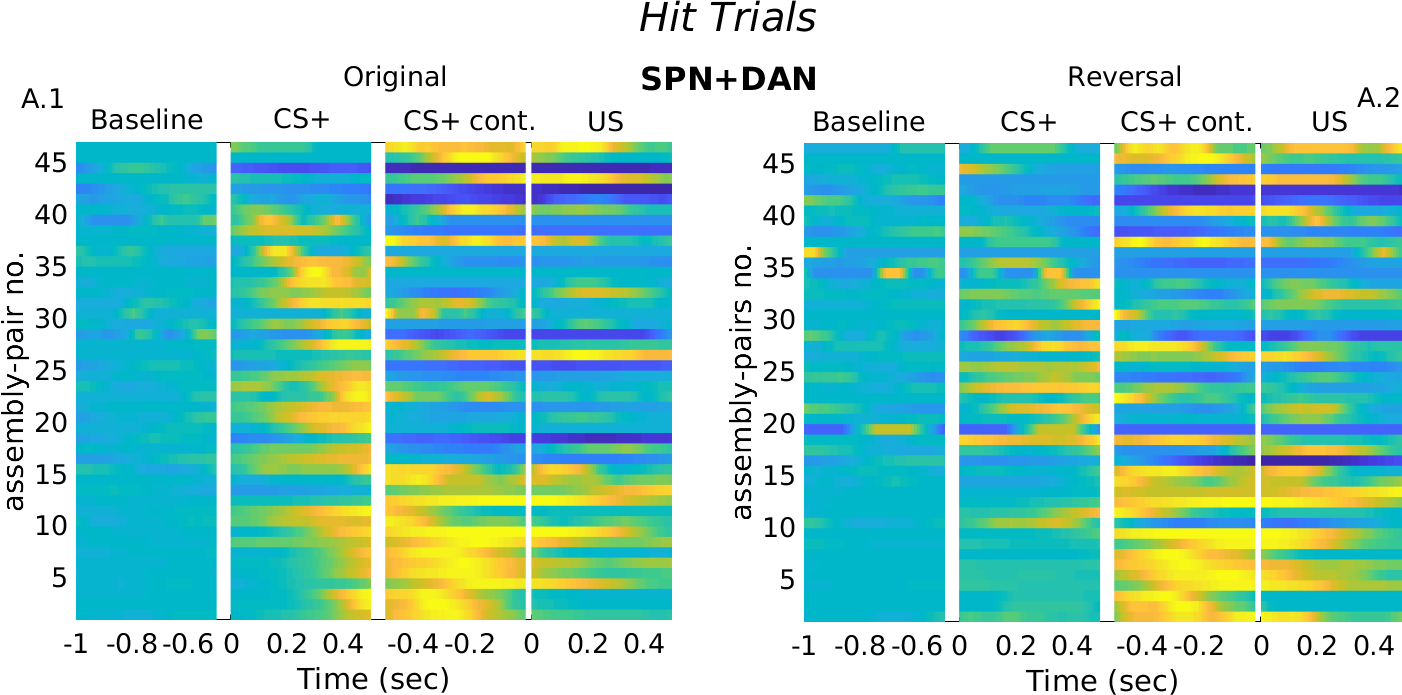
\includegraphics[scale=0.33]{figures/SPN_DANHit.png}
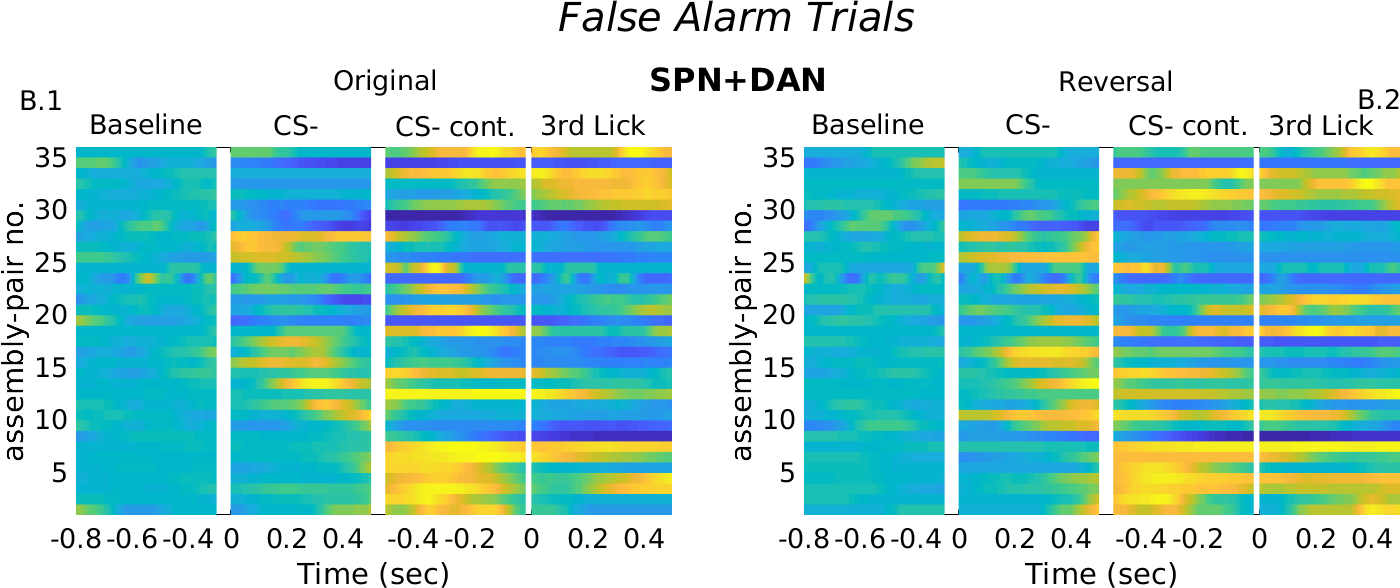
\includegraphics[scale=0.33]{figures/HeatFA_SPN_DAN.png}
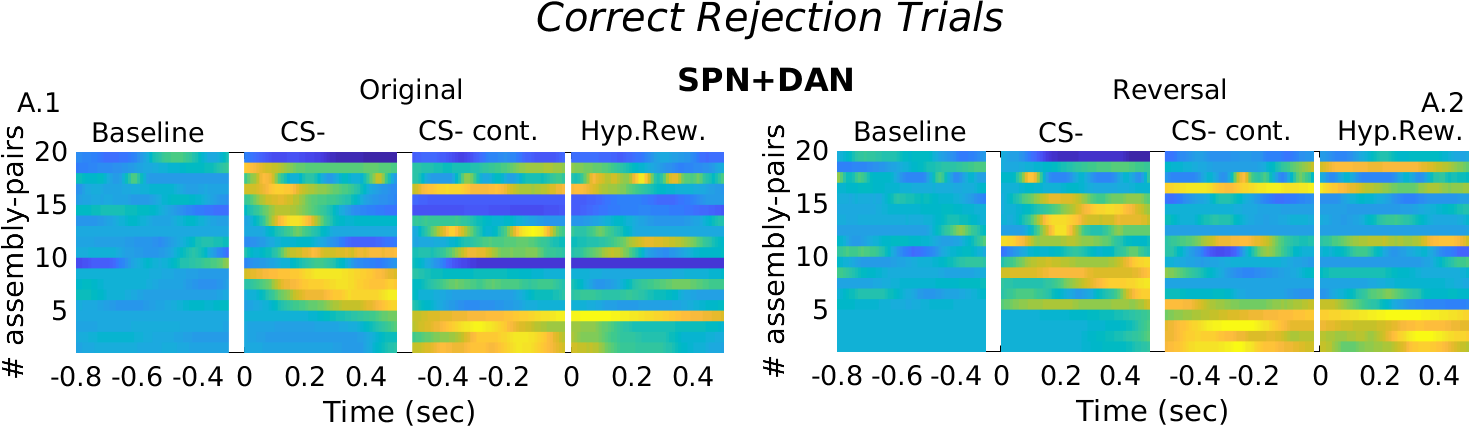
\includegraphics[scale=0.33]{figures/HeatCR_SPN_DAN.png}
\caption{Heat map of significant activation of SPN-DAN assembly-pairs (Friedman test) in three trial segments (Hit, False Alarm and Correct Rejection). In Correct Rejection trials much less assembly-pairs are significant. SPN-DAN assembly-pairs preferentially code for the rewarded odor. The activity of each assembly was normalized as in eq.\ref{eq:norm} were $\max(I)$ ($\min(I)$) was the absolute maximum (minimum) of assembly-activity among the four windows.}
\label{fig:HeatSPN_DANComp}
\end{figure}
\begin{figure}[H]
    \centering
    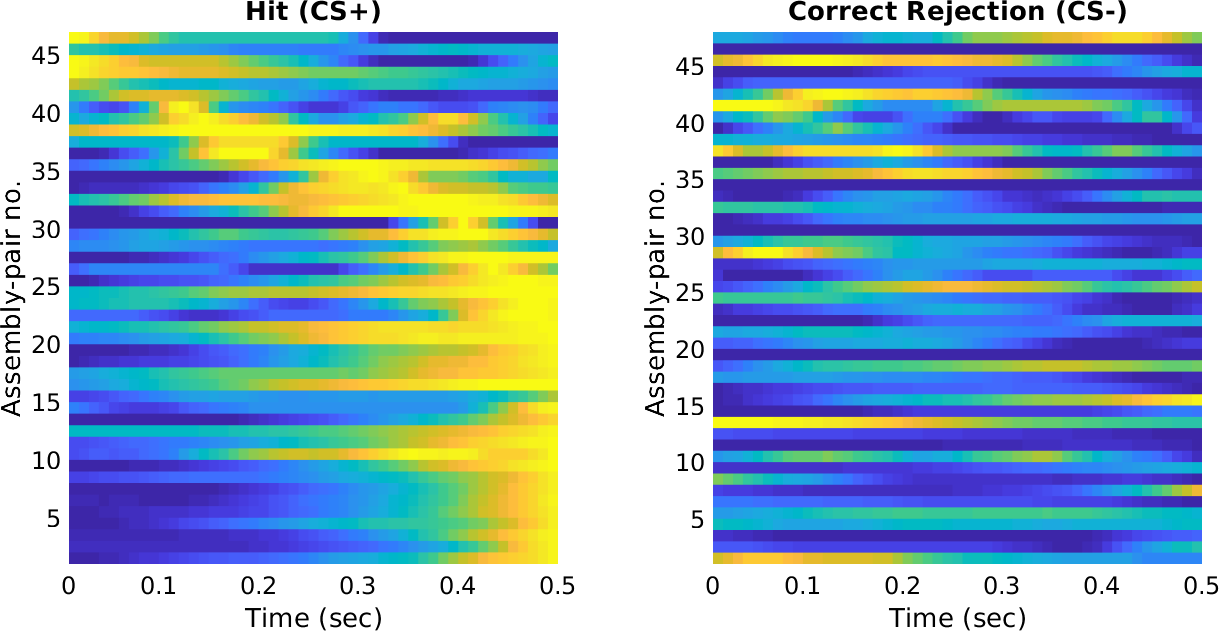
\includegraphics[scale=0.41]{figures/SD_HitCorrRejComp.png}
    \caption{Heat map of significant activation of SPN-DAN (Friedman test in Hit trials), in Hit and Correct Rejection trials. The activity of each assembly was normalized as eq.\ref{eq:norm} were $\max(I)$ ($\min(I)$) was the absolute maximum (minimum) of assembly-activity in the two windows.}
    \label{fig:SD_HitCorrComp}
\end{figure}
Figure \ref{fig:Overlap} shows the fraction of assembly-pairs significant solely in the Hit trials or in both Hit and Correct Rejection trials. Of SPN-DAN assembly-pairs significant for Hit trials in any window  with respect to the baseline the $25\%$ was significant in Correct Rejection trials as well, and only the $12\%$ showed a stimulus related activity compatible with the Hit trials activity. This overlap between Hit trials and Correct Rejection trials was instead strong in FSN-DAN assembly-pairs ($68\%$). These results indicated that FSN-DAN pairs unspecifically respond to the stimulus. 
\begin{figure}
    \centering
    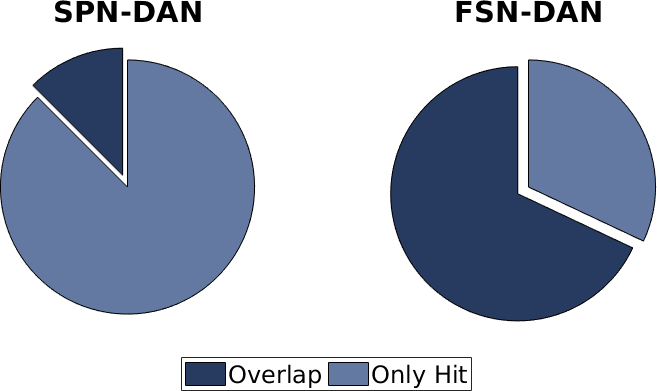
\includegraphics[scale=0.5]{figures/HItCorrRejPieOverlapSD_FD.png}
    \caption{Assembly-pairs significant in Hit trials divided in the fractions significant during CS+ only in Hit trials and in Hit and Correct Rejection trials. \textbf{Left:} SPN-DAN assembly-pairs. \textbf{Right:} FSN-DAN assembly-pairs.}
    \label{fig:Overlap}
\end{figure}
\subsection{FSN-DAN pairs}
FSN-DAN assembly-pair activity patterns were more diverse in their task dependent activation patterns, consistent with the hypothesis that they are unselective to the stimulus type and multisensory in response. In Hit trials (figure \ref{fig:HeatFSN_DANComp}, boxes A.1, A.2) the stimulus (CS+) lead an early activation, early activations could be associated the detection of the signal (see discussion\hyperref[chap:Conclusion]{~Chapter\ref*{chap:Conclusion}}). In Hit trials more than $50\%$ of FSN-DAN pairs phasic activate during the retrieval (US), suggesting that those pairs are not involved in the prediction reward signal. The phasic activation could correspond a lick-related activity or a hedonic signal. In False Alarm and Correct rejection trials (figure \ref{fig:HeatFSN_DANComp}, boxes B.1, B.2, C.1, C.2) the stimulus, unrewarded in this case (CS-), led to an activation of the majority of FSN-DAN pairs, both in original and reversal phase. As shown in figure \ref{fig:Overlap} the identities of those pairs activated by the stimulus in Hit trials overlapped most of the time with those active in Correct Rejection trials, proving that the activation to the stimulus is not a reward related predictive signal. This rather unspecific salience could correspond motivational salience signal and hedonic signals as we expected for VP units.\\We note that of FSN-DAN pairs were sparsely inhibited; particularly in False Alarm and Correct Rejection trials. This inhibition could be again related to motivational factors, such as $"$disappointment$"$. %In the windows before and after the expected reward (CS-$_{cont.}$, 3rd Lick) a good portion ($\sim50\%$) of FSN-DAN assembly-pairs show depression when the reward was predicted but it does not occur, probably coding for the frustration for realizing there will not be a reward, or some negative emotion.\\
%One could observe that an inhibition was observed also in dopamine neurons when the reward was predicted and no reward occurred (see figure \ref{fig:RewardDoya1}, panel A, bottom), however in classical dopamine neurons activity the depression occurs in correspondence of the expected reward, while in FSN-DAN assembly-pairs the inhibition is rather anticipated in False Alarm trials, suggesting that they are involved in a different type of coding that is not, or at least only partially, represented by the classical reward prediction error definition used in reinforcement learning models.\\
%FSN-DAN assembly-pairs reward-related answer is rather unspecific and difficult to interpret. However FSN-DAN assembly-pairs activity could be specific in other aspects of mediation of experience-dependent behavior, such as the motivational salience either at the odor presentation, or at the choice.\\Finally we show FSN-DAN activity patterns in Correct Rejection trials (figure \ref{fig:HeatFSN_DANComp}, boxes C.1, C.2): here we observe that a good portion of FSN-DAN assembly-pairs is early positively activated by the stimulus presentation (CS- window), another group ($\sim30\%$ of assembly-pairs) is instead inhibited. This depression can be interpreted as codification of the disappointment of the animal when the recognized unrewarded odor is presented, furthermore the $\sim10\%$ of assembly-pairs show an inhibitory response in CS-$_{cont.}$ window, after an excitation in CS- interval.
 \begin{largefigure}[17pt]
 \centering
 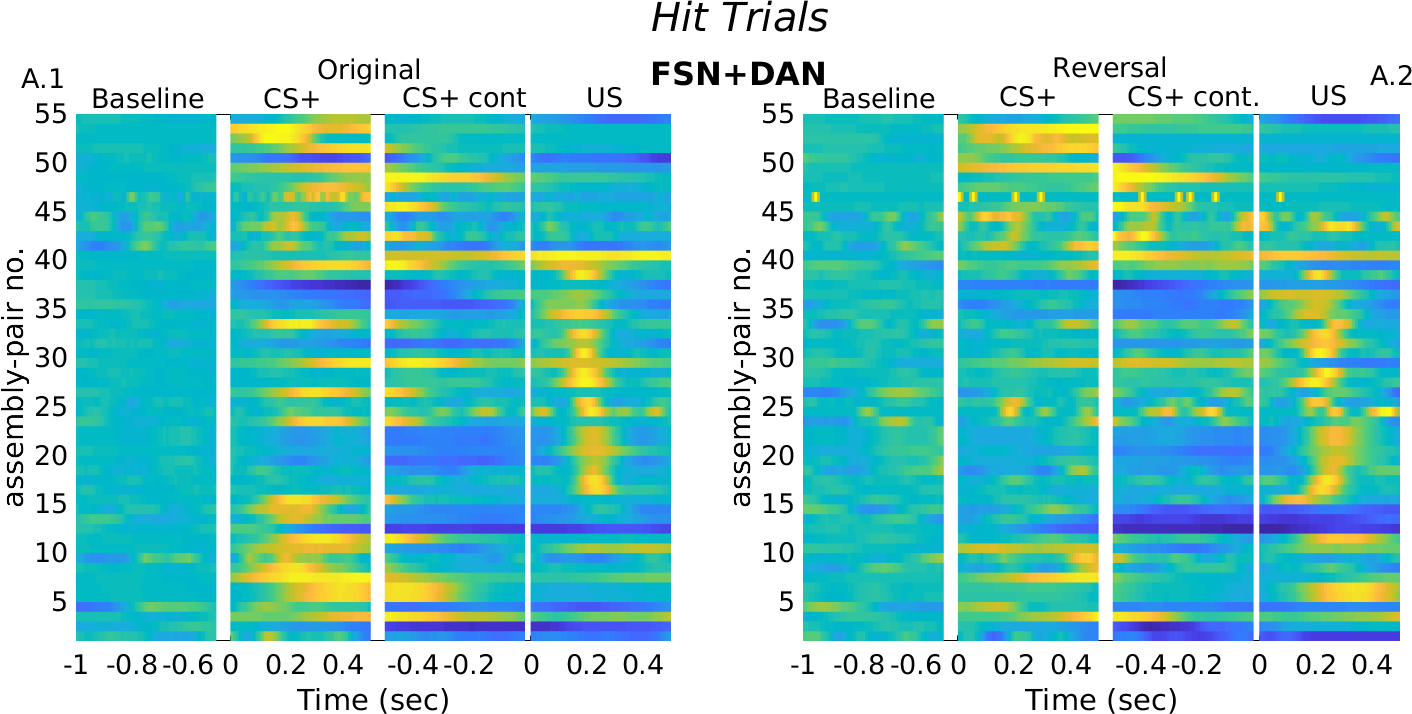
\includegraphics[scale=0.34]{figures/HeatFSN_DANHit1.png} 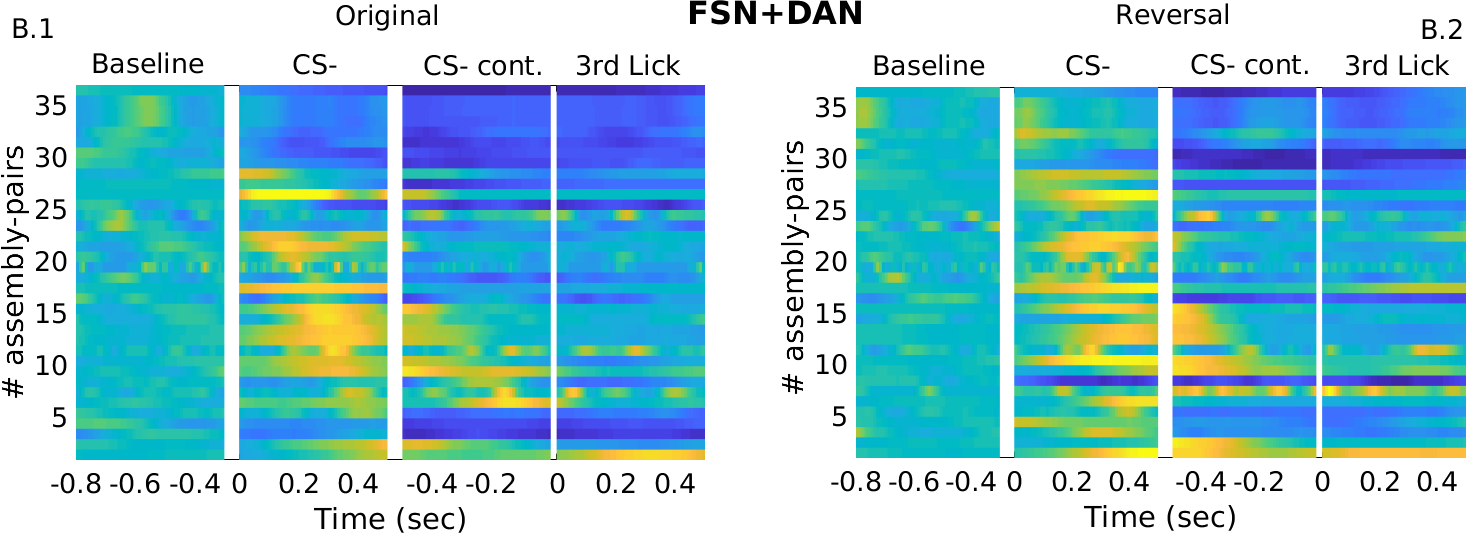
\includegraphics[scale=0.34]{figures/HeatFA_FSN_DAN.png}
 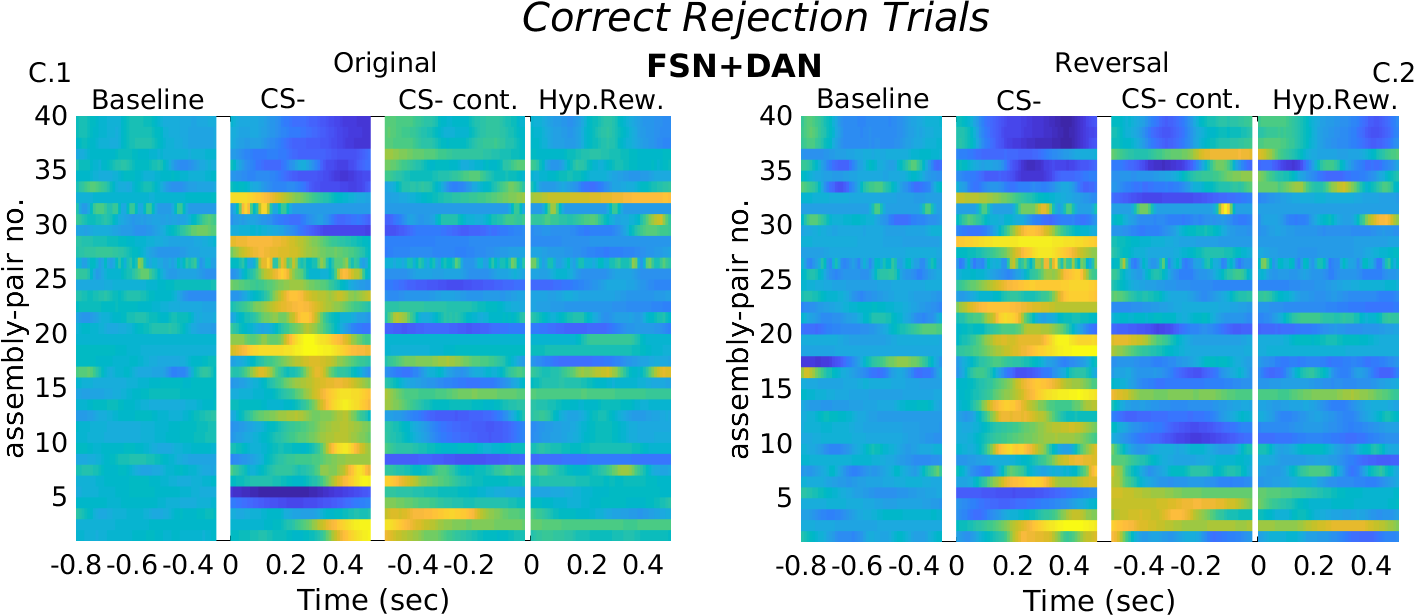
\includegraphics[scale=0.34]{figures/HeatCR_FSN_DAN.png}
  \caption{Heat map of significant activation of FPN-DAN (Friedman test). FSN-DAN assembly-pair activity patterns are diverse in their task dependent activation pattern. In Hit trials (A.1, A.2) early stimulus (CS+) response and a phasic response on retrieval (US). In False Alarm trials (boxes B.1, B.2) and Correct Rejection trials (boxes C.1, C.2) the activation to the stimulus remains, no excitatory activation in the windows before and after the expected reward time.}
  \label{fig:HeatFSN_DANComp}
\end{largefigure}
%\begin{figure}
 %   \centering
   % 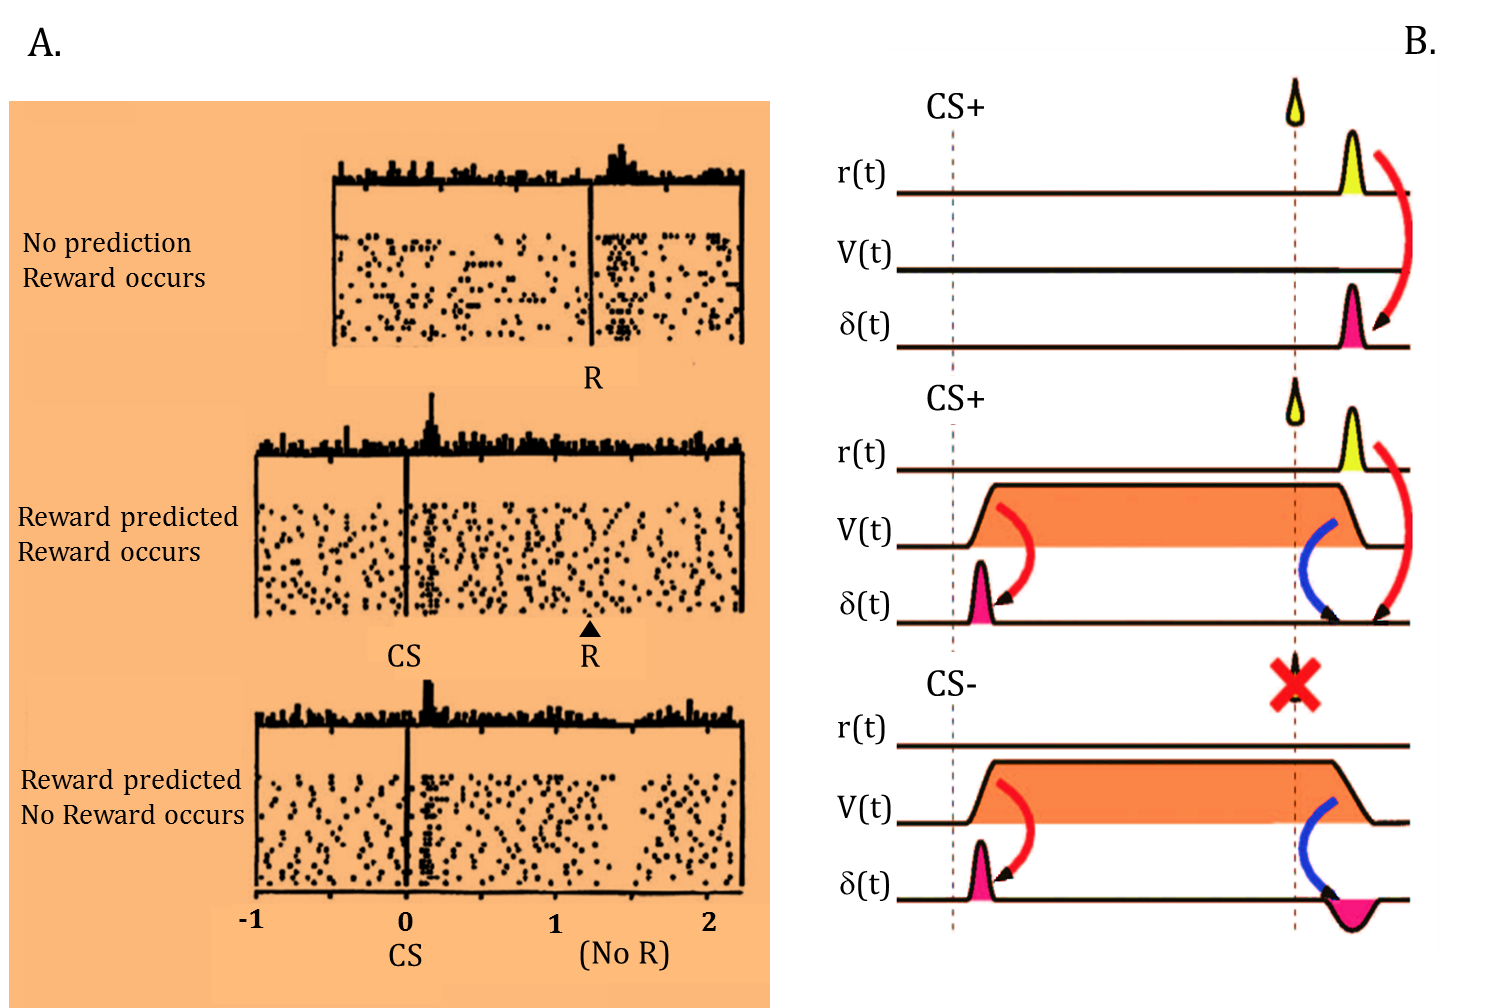
\includegraphics[scale=0.5]{figures/RewardDoyaRLSUM.png}
  %  \caption{Adapted from \cite{Doya}. In the first two panels response associated to rewarded trials. Last panel is related to unrewarded trials, in the cases in which the reward was predicted but it did not occur. Activity of the dopamine neuron is depressed exactly at the time when the reward would have occurred.}
 %   \label{fig:RewardDoya1}
%\end{figure}
%\pagebreak

\section{Conclusion}
In the previous two sections we described the task-related activity of assembly-pair types. We first noticed that different assembly-pairs types showed different task-related patterns of activity, and consequently they could exhibit different coding features.\\The observed activity patterns, at the stimulus presentation and at the retrieval, revealed that VS-VTA pairs were encoding difference between expected and received outcomes.\\ 
%Typical single neuron activity in VS and VTA related to expectancy of reward and uncertainty was largely investigated in last decades (\cite{Fiorillo}, \cite{Schultz}, \cite{Schultz1992}, \cite{Schultz1998}), however how the VS-VTA interaction could form and encode those kind of signals is not fully understood. As first step we made a parallelism between the single unit activity related to probability of reward and the activity exhibited by the detected assembly-pairs.\\
In particular from the resemblance of SPN-DAN responses to the rewarded stimulus and expected for prediction error signals, we generated the hypothesis that SPN-DAN assembly-pairs encode prediction signals.\\To prove the aforementioned hypothesis we introduce the learning dynamic in our analysis, through a reinforcement learning model. The prediction signal is indeed considered to be the basis of associative learning (\cite{RescorlaWagner}), and bears a striking resemblance to machine learning algorithms (\cite{SuttonBarto}).\\Despite FSN-DAN pairs seemed to not encode the main component of prediction error, they show differential activity in Hit, False Alarm and Correct Rejection trials. However, the unselective and multisensory nature of their response could correspond to a braod range of coding futures, that do not look prediction error specific, rather motivational salience and hedonic signal as one expects for VP (\cite{Root}).\\ Motivation components are barely explained by the classical reward prediction error signal as parameterized in reinforcement learning model, hence we use FSN-DAN pairs as control in the reinforcement learning model.
%In Hit trials the rewarded stimulus leads an early phasic activation, that could correspond the detection component of prediction error signal. Furthermore those pairs show a phasic response at retrieval that could correspond a lick- related activity or a hedonic signal. The inhibition in False Alarme and Correct Rejections suggested as well an involvement in some outcome-related feelings or choice (lick, no-lick) execution-related activation, which reflects in turn motivational components.\\
 %%%%%%%% Commento forse da buttare
 %First difference between original and reversal phase is number of assemblies responding during the post-stimulus interval, this number decrease for all the typologies involved during hit trials (as shown in figure  (\ref{fig:histo_taskrel})), in according to the intuition, in reversal phase in fact, when the animals became more expert, neuronal response tend to be shifted closer to the reward delivery. This effect can be seen in figure  (\ref{fig:NeusInAsse}) where activity and raster plots of two units in a pair are shown. Looking at the raster plots, a shift in correspondence to the phase-switch is evident in both units.
 %\begin{figure}
  %   \centering
  %   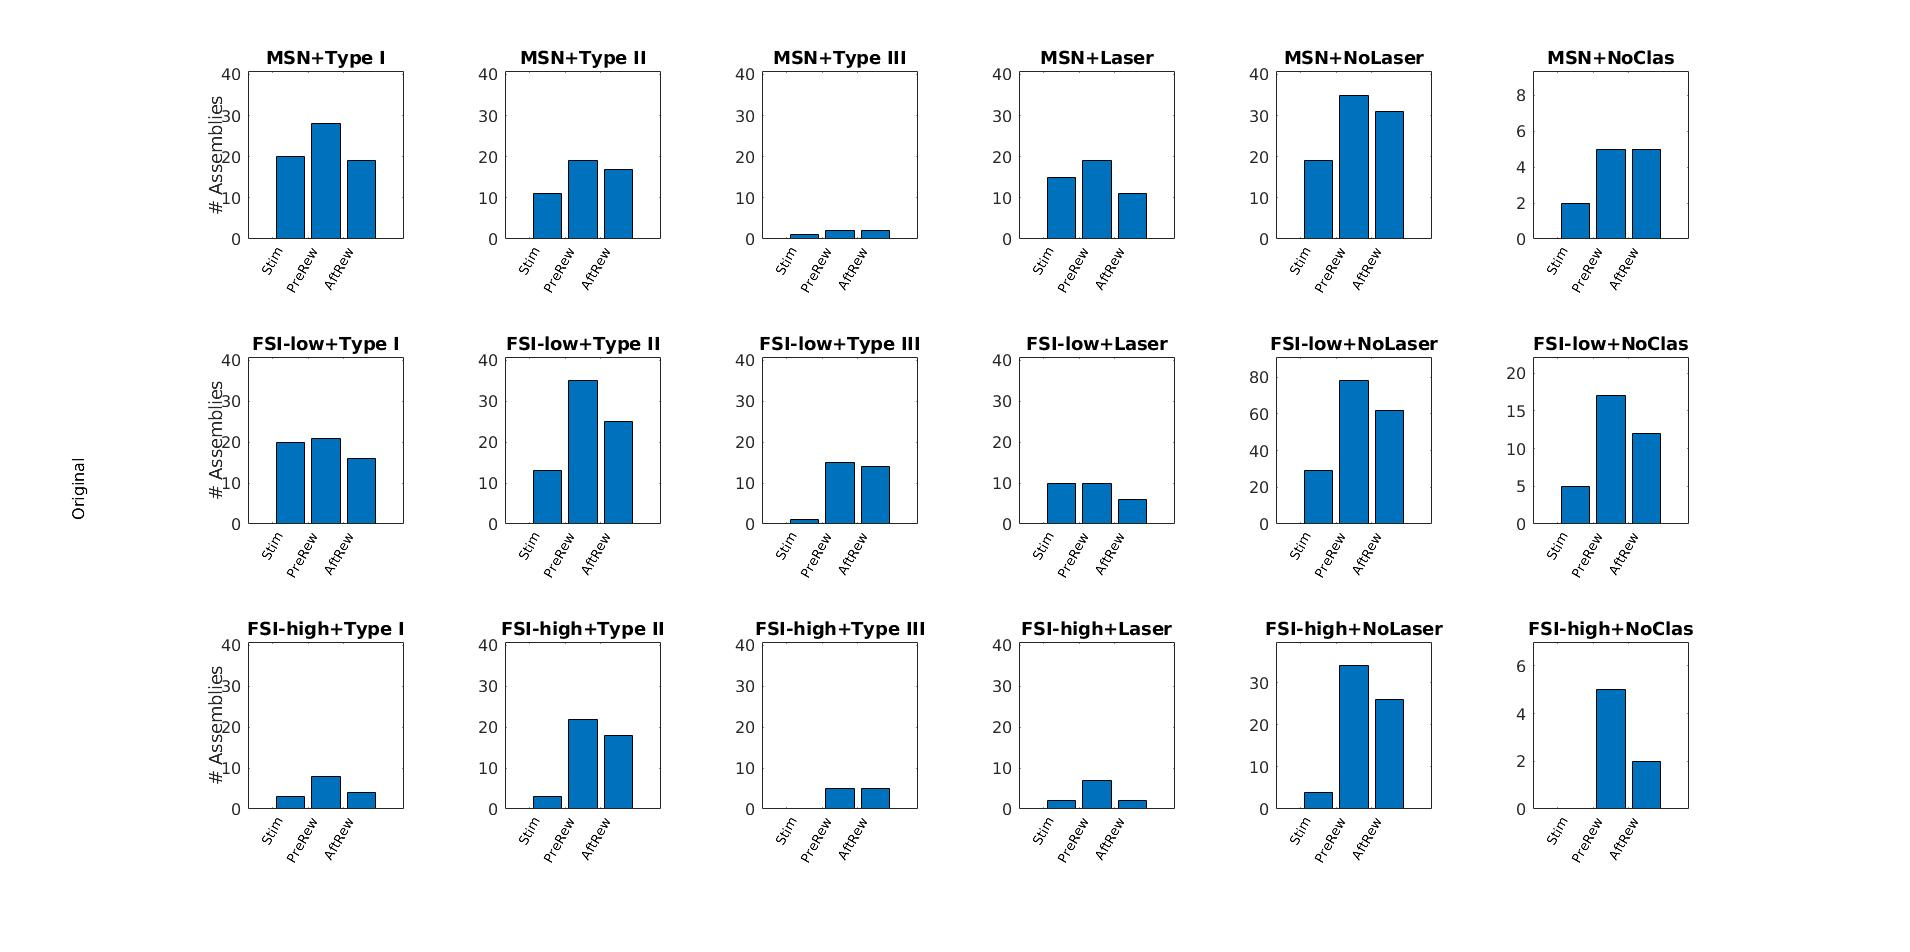
\includegraphics[scale=0.3]{figures/Original_Hit_N.jpg}
    % 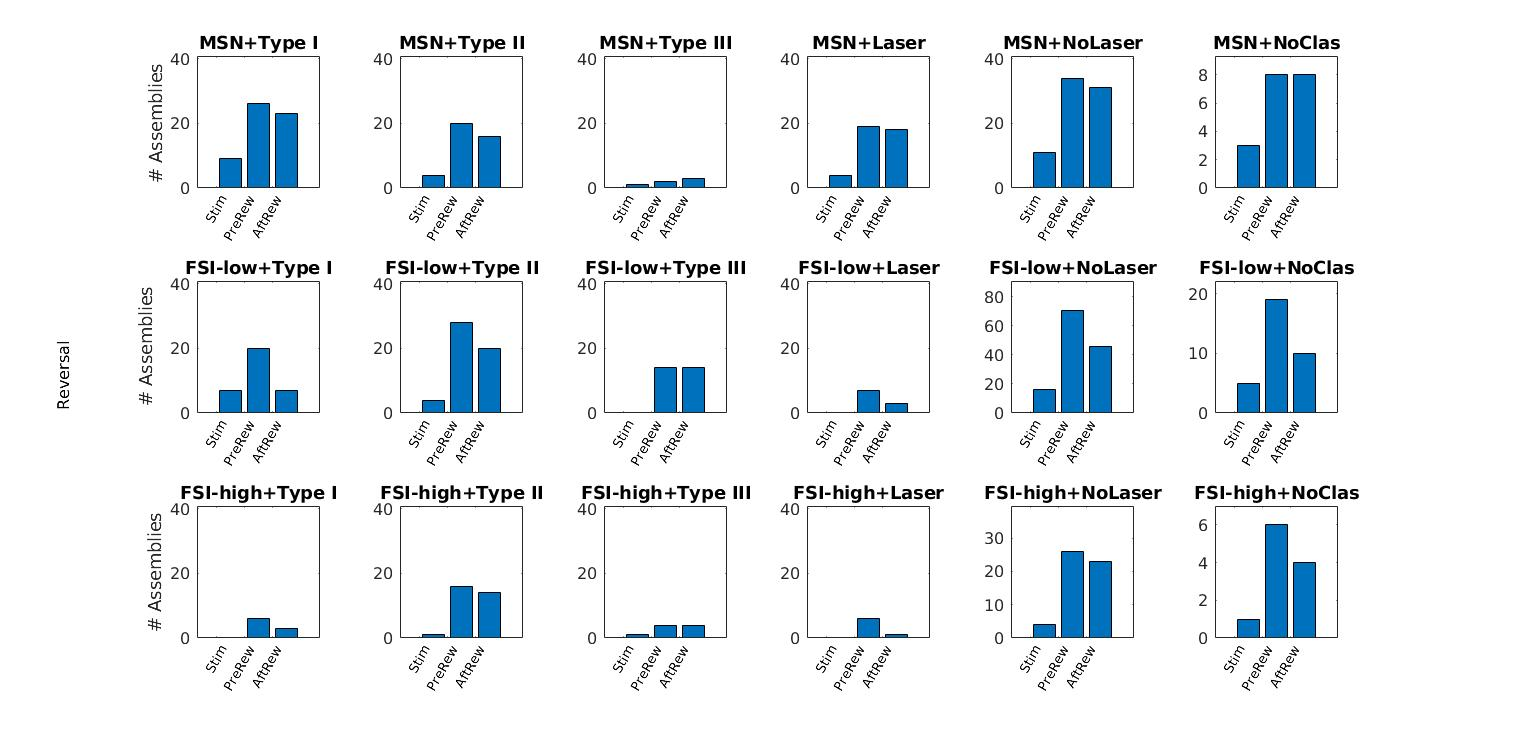
\includegraphics[scale=0.3]{figures/Reversal_Hit_N.jpg}
     %\caption{{\color{red}TO MODIFY!!!! BUT THIS IS THE PLOT}}
     %\label{fig:histo_taskrel}
 %\end{figure}
%\begin{figure}
  %  \centering
   % 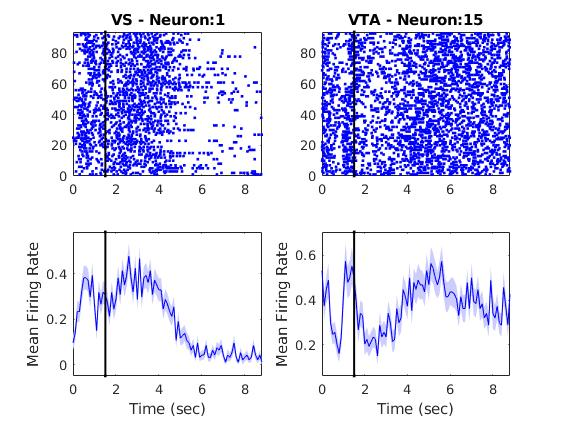
\includegraphics[scale=0.6]{figures/SingleNeus1_15Lastrev1Pru_An_4.jpg}
    %\caption{Shift in time of neuronal activity of two units in assembly. }
    %\label{fig:NeusInAsse}
%\end{figure}

%\section{Discussion}
%\section{Combination of single neuron and assemblies analysis}
%\subsection{Directionality using classification}
%\subsection{Significant task related response for typology}
%%%%%%% Fine Commento forse da buttare


%%%%% Commento Utile
%To better study assemblies activation patterns, first the task relevant moments of the experiment were selected. From the mean task related activity patterns we expected to see differences among assemblies types in two experimental chapters (original and reversal). To better visualize the task related activation patterns via heat plots, hit trials (rewarded odor, mouse went for reward), correct rejection trials (unrewarded odor, mouse sat quiet), false alarm trials (unrewarded odor, mouse went for reward), were kept separated; however this separation among trials types was released in further analysis, without affecting results.
%The assemblies were pruned according their significant task related activity, that was tested with Friedman's test and a non parametric version of the repeated measures Anova. We preferred to use non-parametric tests to be free from the assumption of gaussianity of the observations. Results of the two tests were consistent each other. The two relevant events of the task were the odor onset and the reward delivery, then we choose whether the assemblies showed a significant activity in three windows: Stimulus [0s, 0.5s], Pre-Reward [-0.5s, 0s], Reward [0s, 05s], the baseline was chosen in the interval [-1s, -0.5s] from the odor onset. Post-hoc analysis were performed using the Bonferroni's criterion {\color{red}check whether the criterion was Bonferroni of some other}. Almost $80\%$ of the VS-VTA assemblies showed a task related activity significant different from the baseline or from another of the windows considered. Of the significant assemblies $\%$ were composed by MSN-Type I units, $\%$ by FSI low-Type I, $\%$ by FSI high-Type I, $\%$ MSN-Type II, $\%$ by FSI low-Type II, $\%$ by FSI high-Type II, the other possible units combinations constitutes a minority and all toghether were the $\%$ {\color{red} Insert numbers of percentage}.

%\section{Conclusion}
